\begin{frame}
	\frametitle{Post-Processing}

	Order of Post-Processing Steps:

	\begin{columns}
		\column{0.5\textwidth}

			\begin{itemize}

				\item
					Path Simplification
					\begin{itemize}
						\item Pose Removal
						\item Corner Removal
					\end{itemize}
			\end{itemize}

		\column{0.5\textwidth}

			\begin{itemize}
				\item Rotation Optimisation using slerp
					\begin{itemize}
						\item Due to sampling strategy, very little optimisation
							required
					\end{itemize}
				\item Smoothing with B-splines

			\end{itemize}


	\end{columns}
		\begin{figure}[hb]
			\centering
			\def\svgwidth{\columnwidth}
			\import{res/img/}{superfluous_poses.pdf_tex}
			\caption{Superfluous Pose Removal}%
			\label{fig:superfluous_poses}
		\end{figure}
\end{frame}

\begin{frame}
	\frametitle{B-Spline Collision Guarantee}
		\begin{figure}[hbt]
			\centering
			\def\svgwidth{\columnwidth}
			\import{res/img/}{knot_multiplicity.pdf_tex}
			\caption{Increasing B-Spline Knot Multiplicity}%
			\label{fig:set_of_poses_augmentation}
		\end{figure}

		\begin{figure}[hbt]
			\centering
			\def\svgwidth{\columnwidth}
			\import{res/img/}{augmented_control_points.pdf_tex}
			\caption{Augmenting Control Points}%
			\label{fig:set_of_poses_augmentation}
		\end{figure}
\end{frame}

\begin{frame}
	\frametitle{B-spline Collision Guarantee with $\setofposes$-Augmentation}

	\begin{itemize}
		\item B-spline used to interpolate poses
		\begin{figure}[hbt]
			\centering
			\def\svgwidth{0.7\columnwidth}
			\import{res/img/}{subdivide_control_points.pdf_tex}
			\caption{$\setofposes$ Augmentation}%
			\label{fig:set_of_poses_augmentation}
		\end{figure}
	\end{itemize}
\end{frame}

\begin{frame}
	\frametitle{B-spline Collision Guarantee with $\setofposes$-Augmentation}
	\begin{center}
		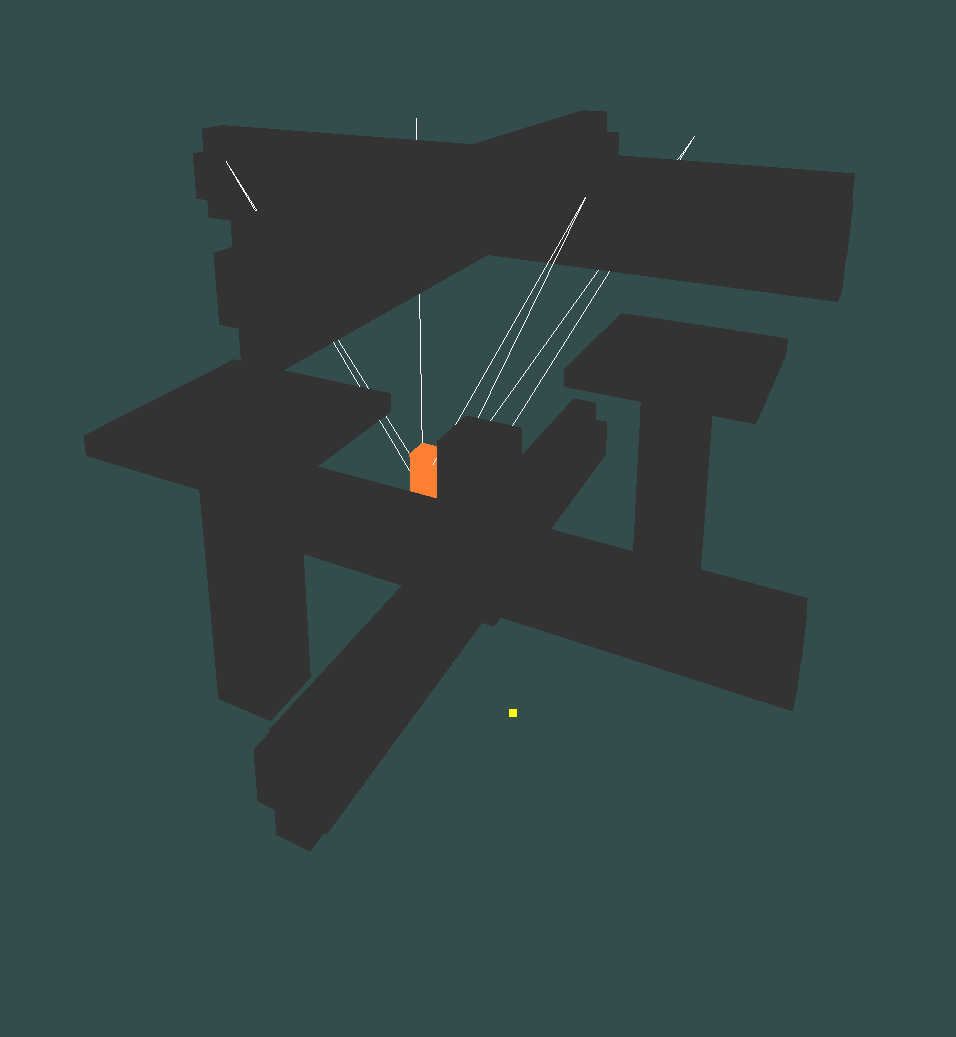
\includegraphics[width=\textwidth, height=0.8\textheight, keepaspectratio=true]{clutter_perspective.png}
		\captionof{figure}{Sample planning problem}
	\end{center}
\end{frame}

\begin{frame}
	\frametitle{B-spline Collision Guarantee with $\setofposes$-Augmentation}

	\begin{columns}

		\column{0.5\textwidth}
			\begin{figure}[hb]
				\centering
				\begin{minipage}{0.8\linewidth}
					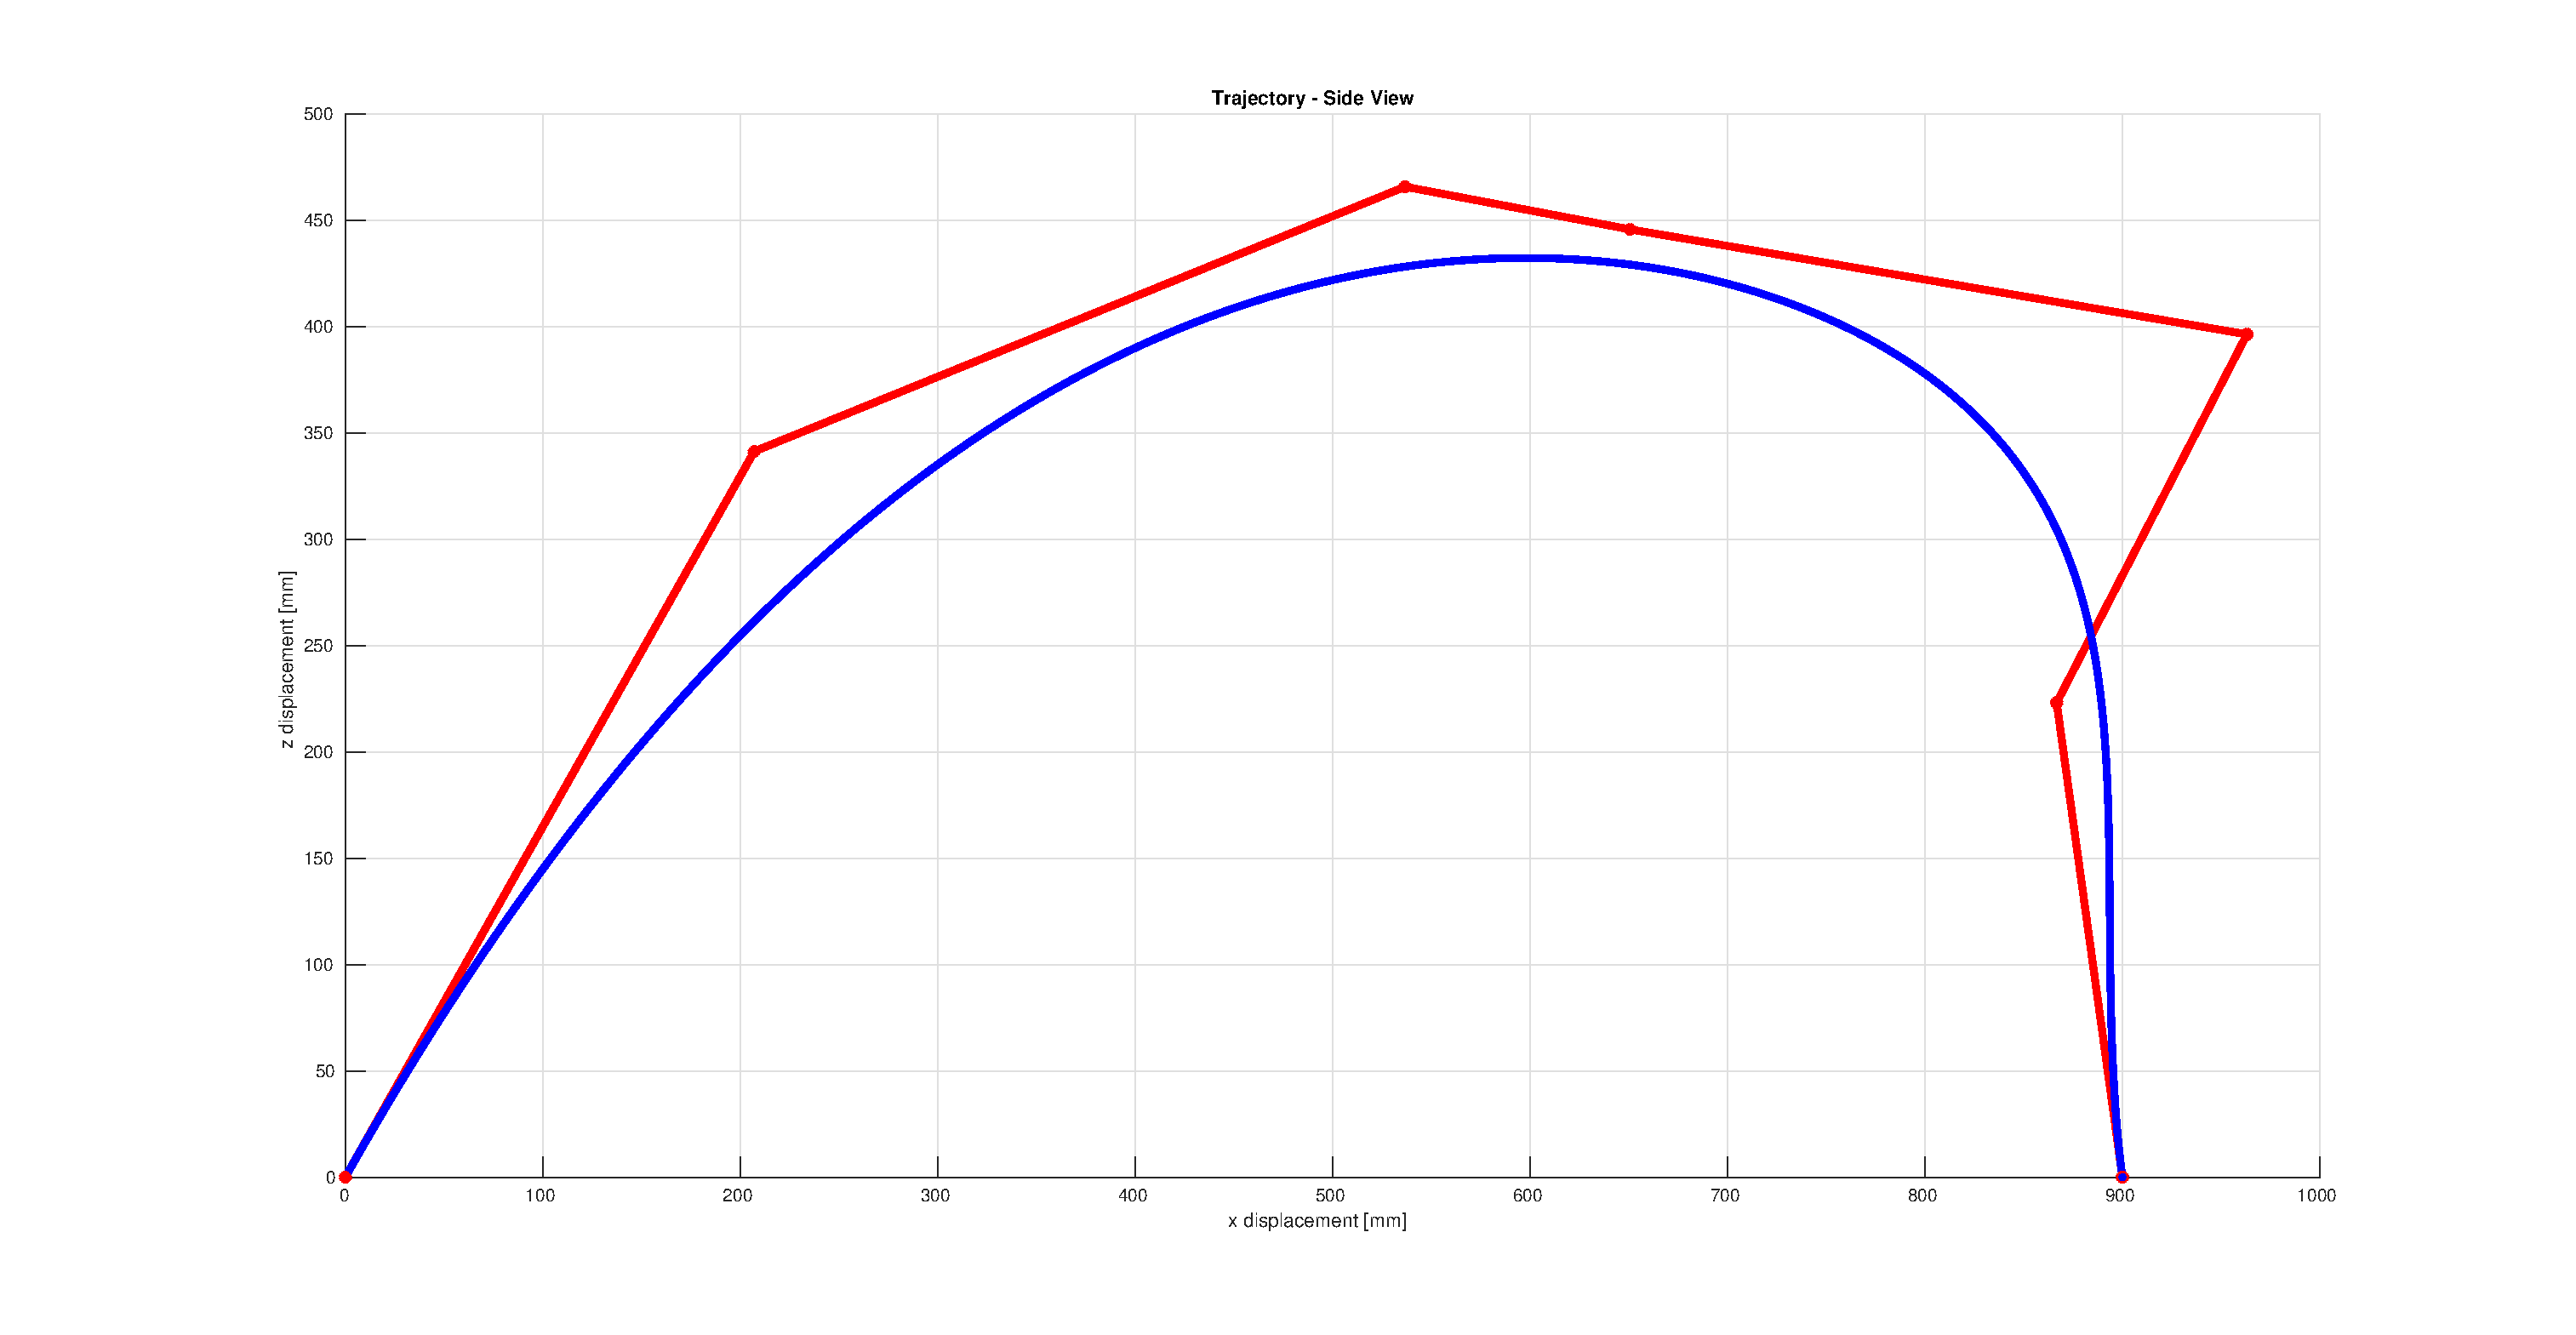
\includegraphics[height=0.45\linewidth, width=0.45\linewidth]{trajectory_simplify_no_subdivide_side.eps}
					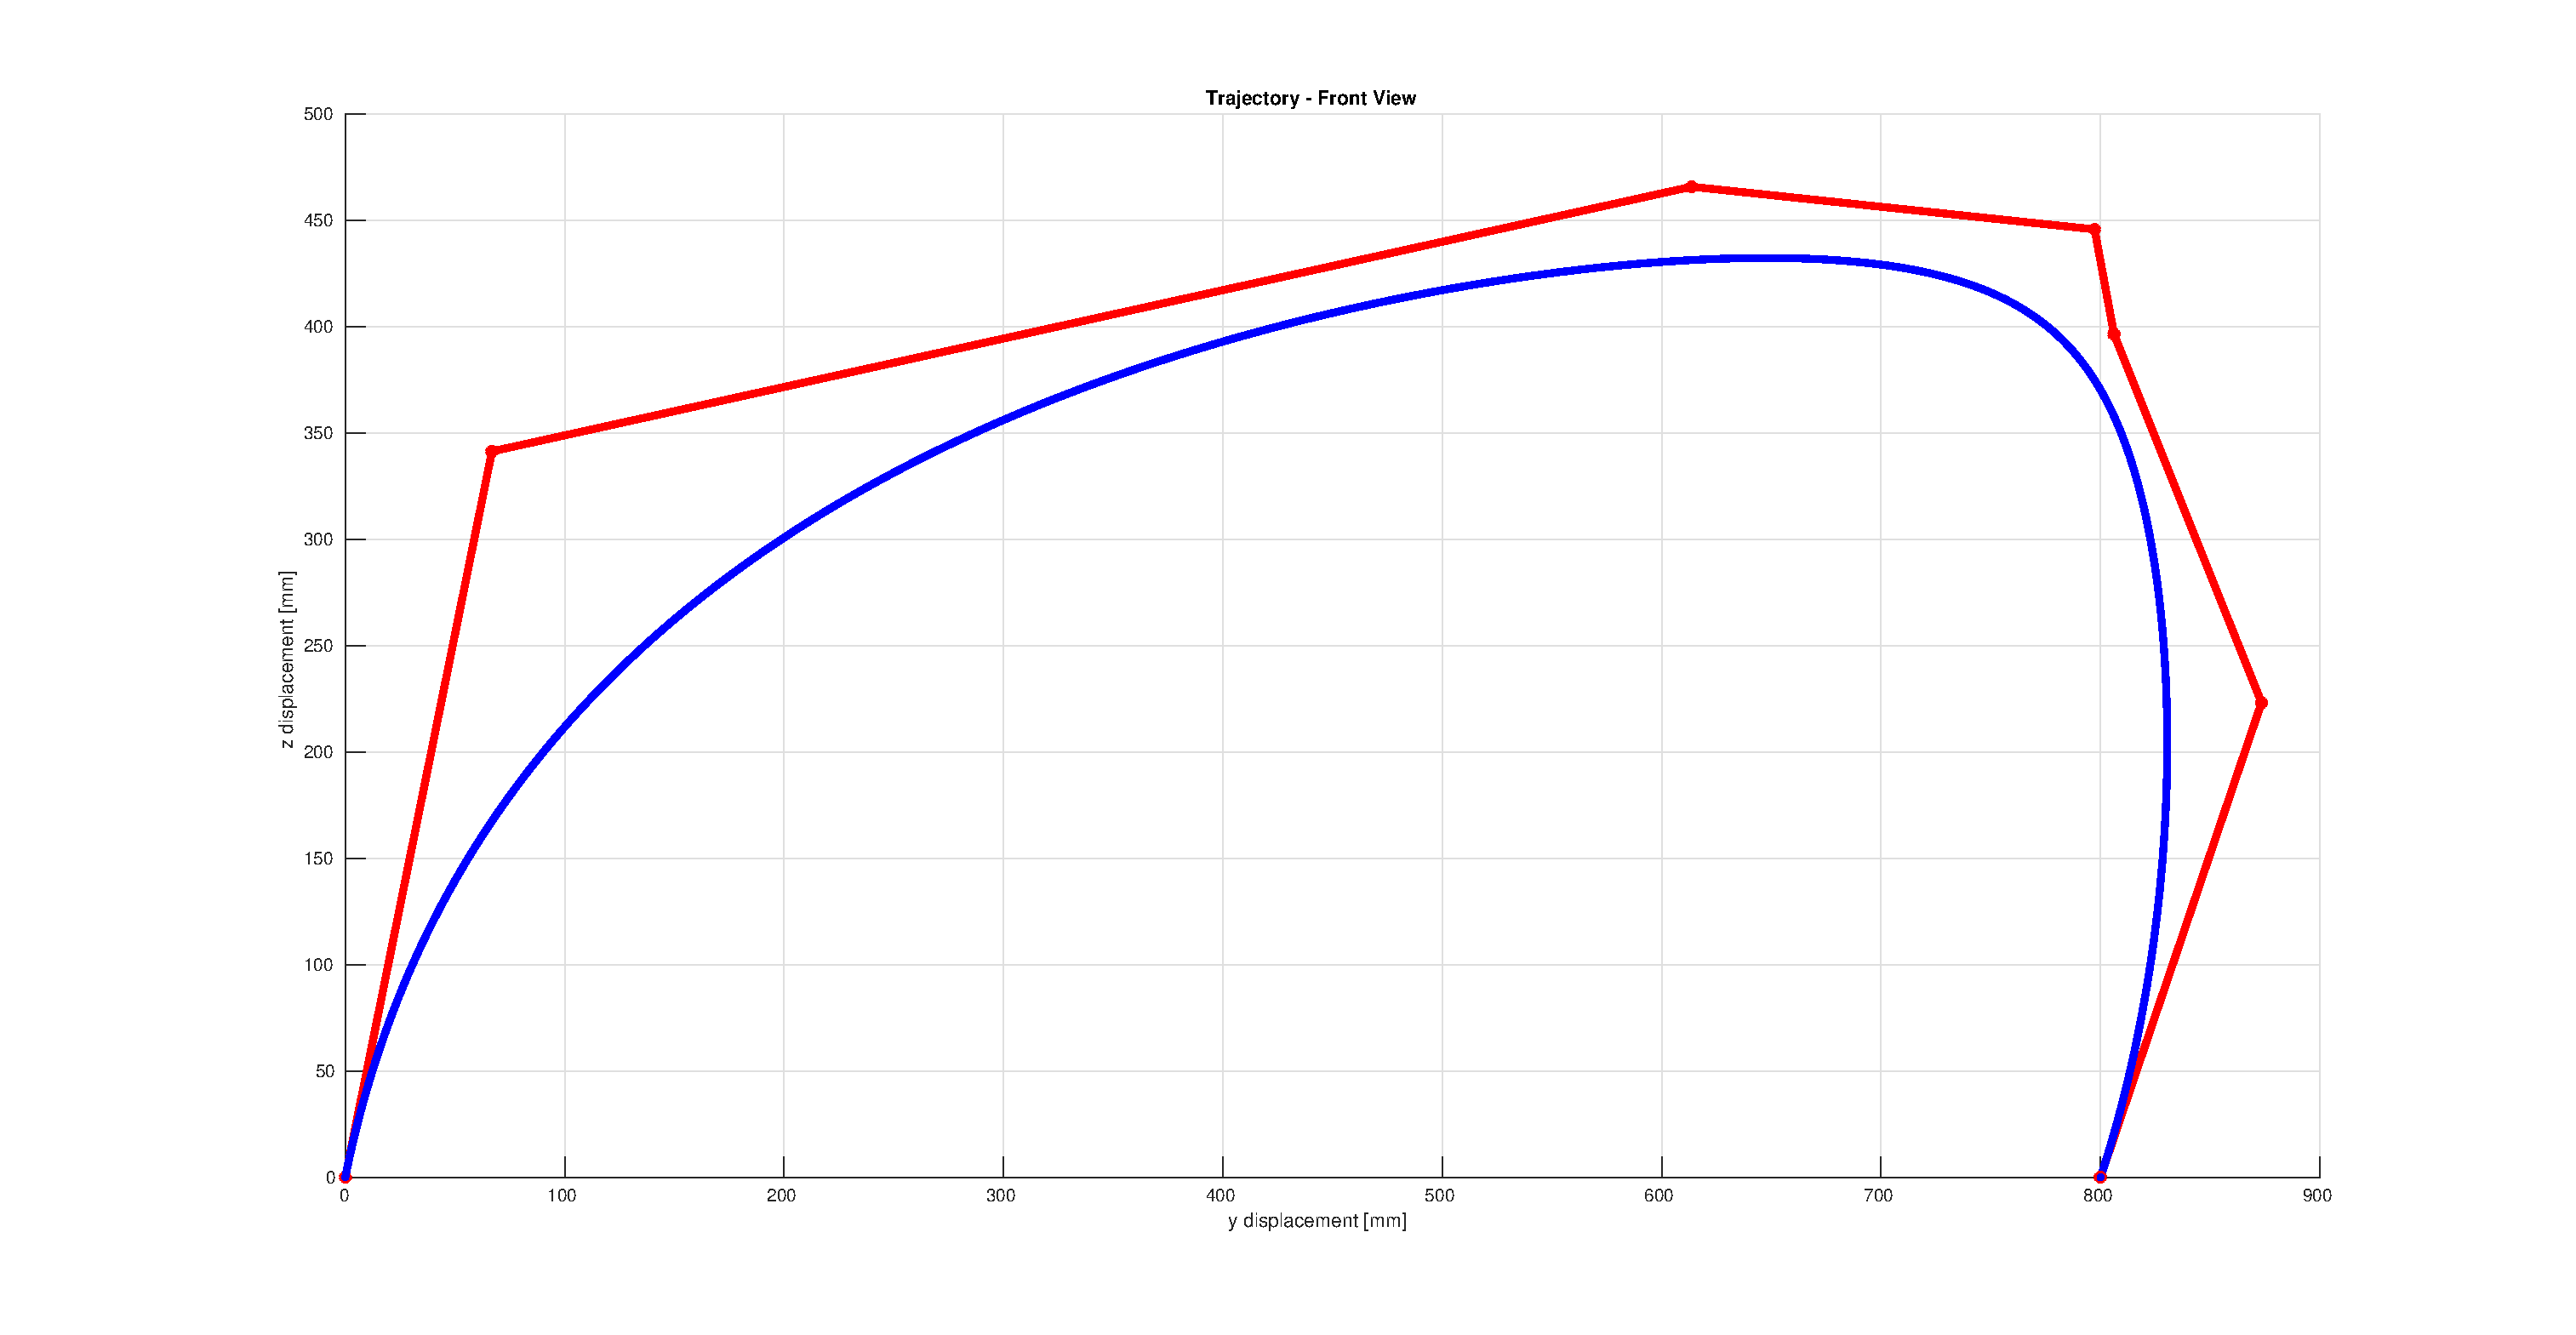
\includegraphics[height=0.45\linewidth, width=0.45\linewidth]{trajectory_simplify_no_subdivide_front.eps}
					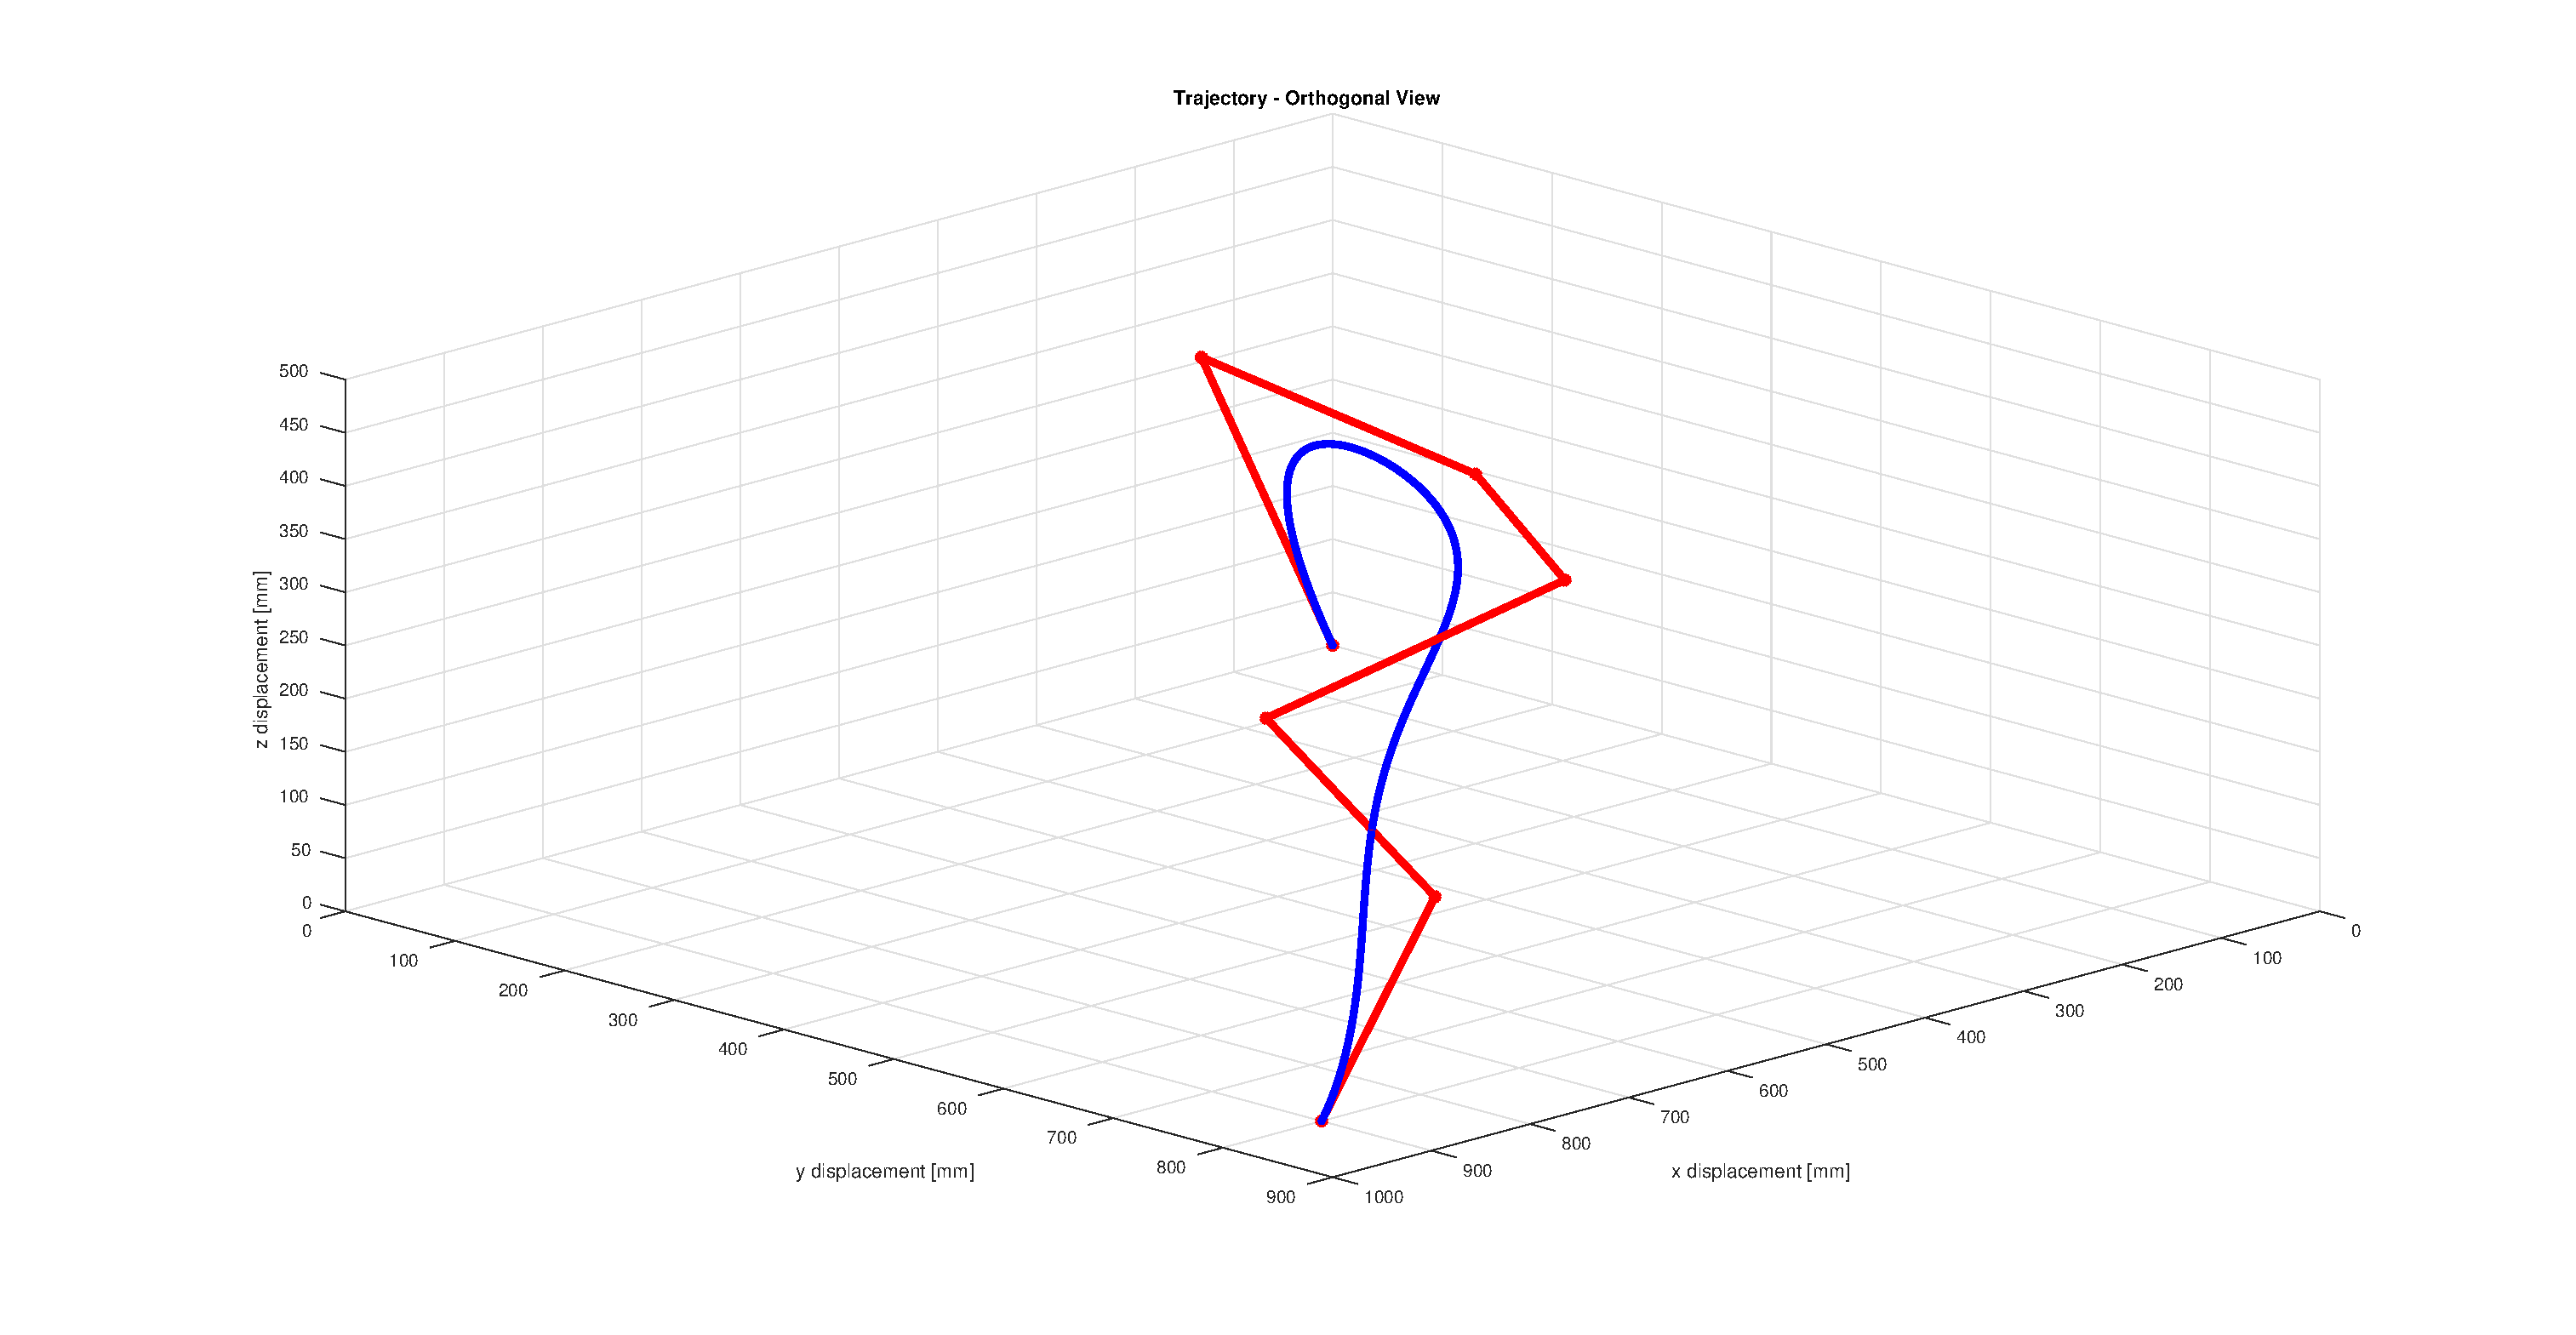
\includegraphics[height=0.45\linewidth, width=0.45\linewidth]{trajectory_simplify_no_subdivide_orthogonal.eps}
					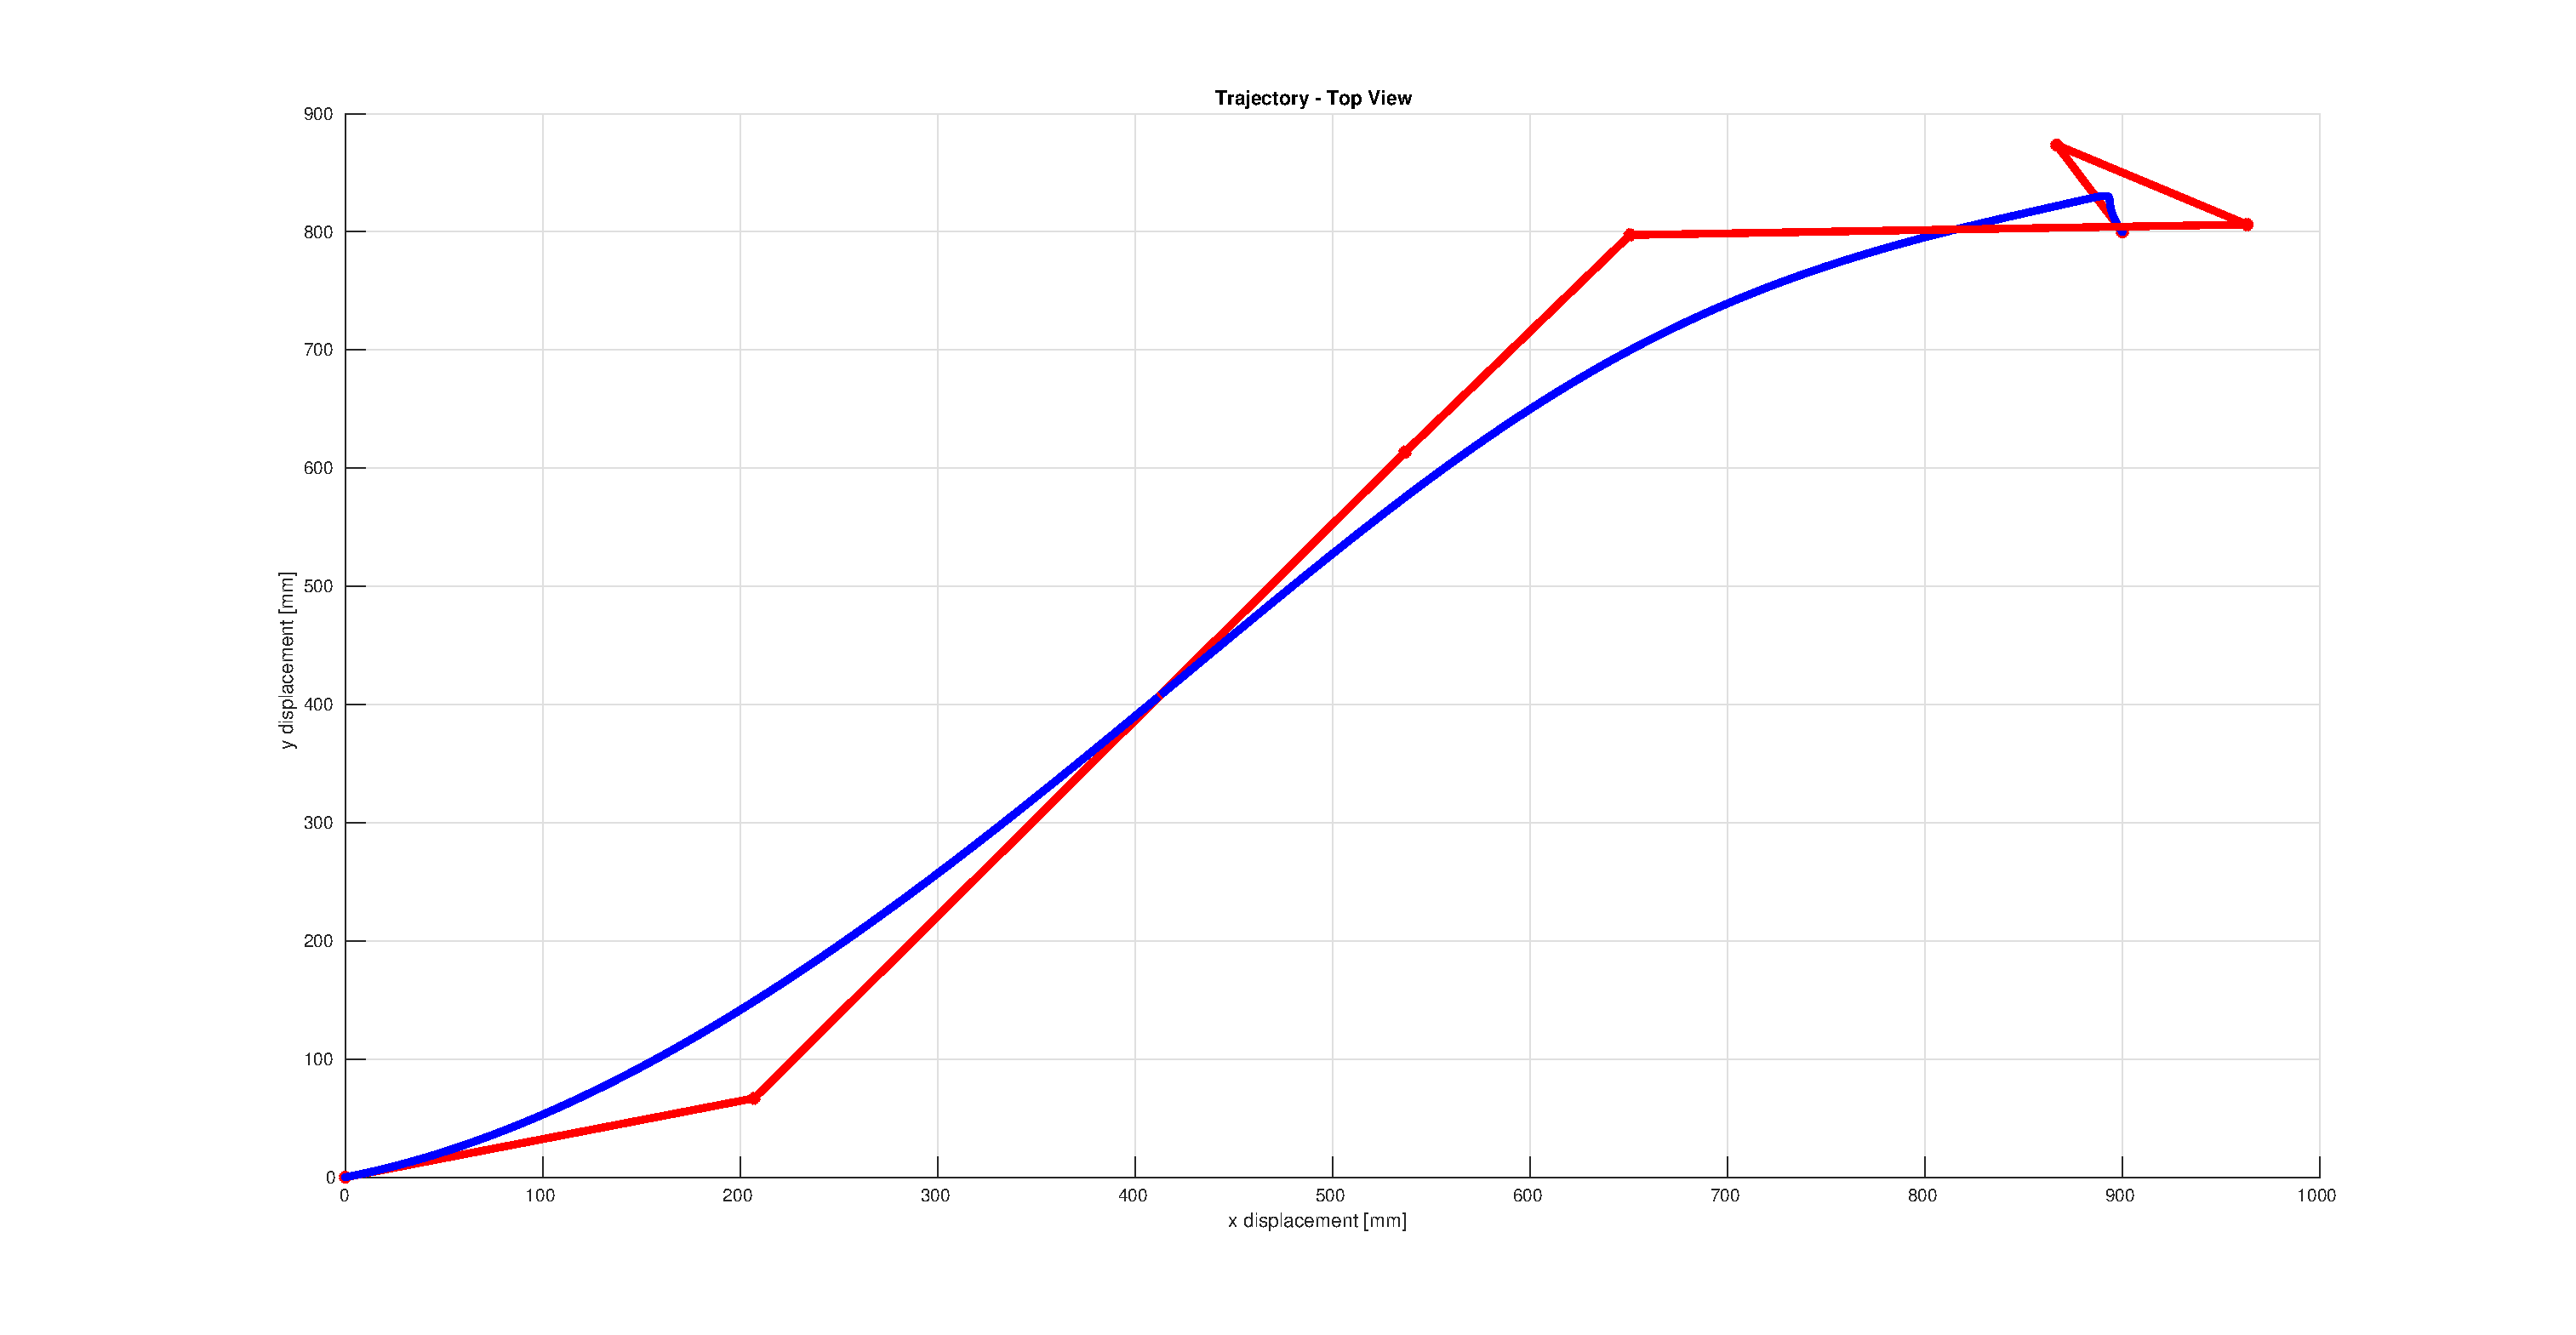
\includegraphics[height=0.45\linewidth, width=0.45\linewidth]{trajectory_simplify_no_subdivide_top.eps}
				\end{minipage}
				\caption{Sample Trajectory without Augmenting $\setofposes$}
				\label{fig:sample_trajectory_after_simplification}
			\end{figure}

		\column{0.5\textwidth}
			\begin{figure}[hb]
				\centering
				\begin{minipage}{0.8\linewidth}
					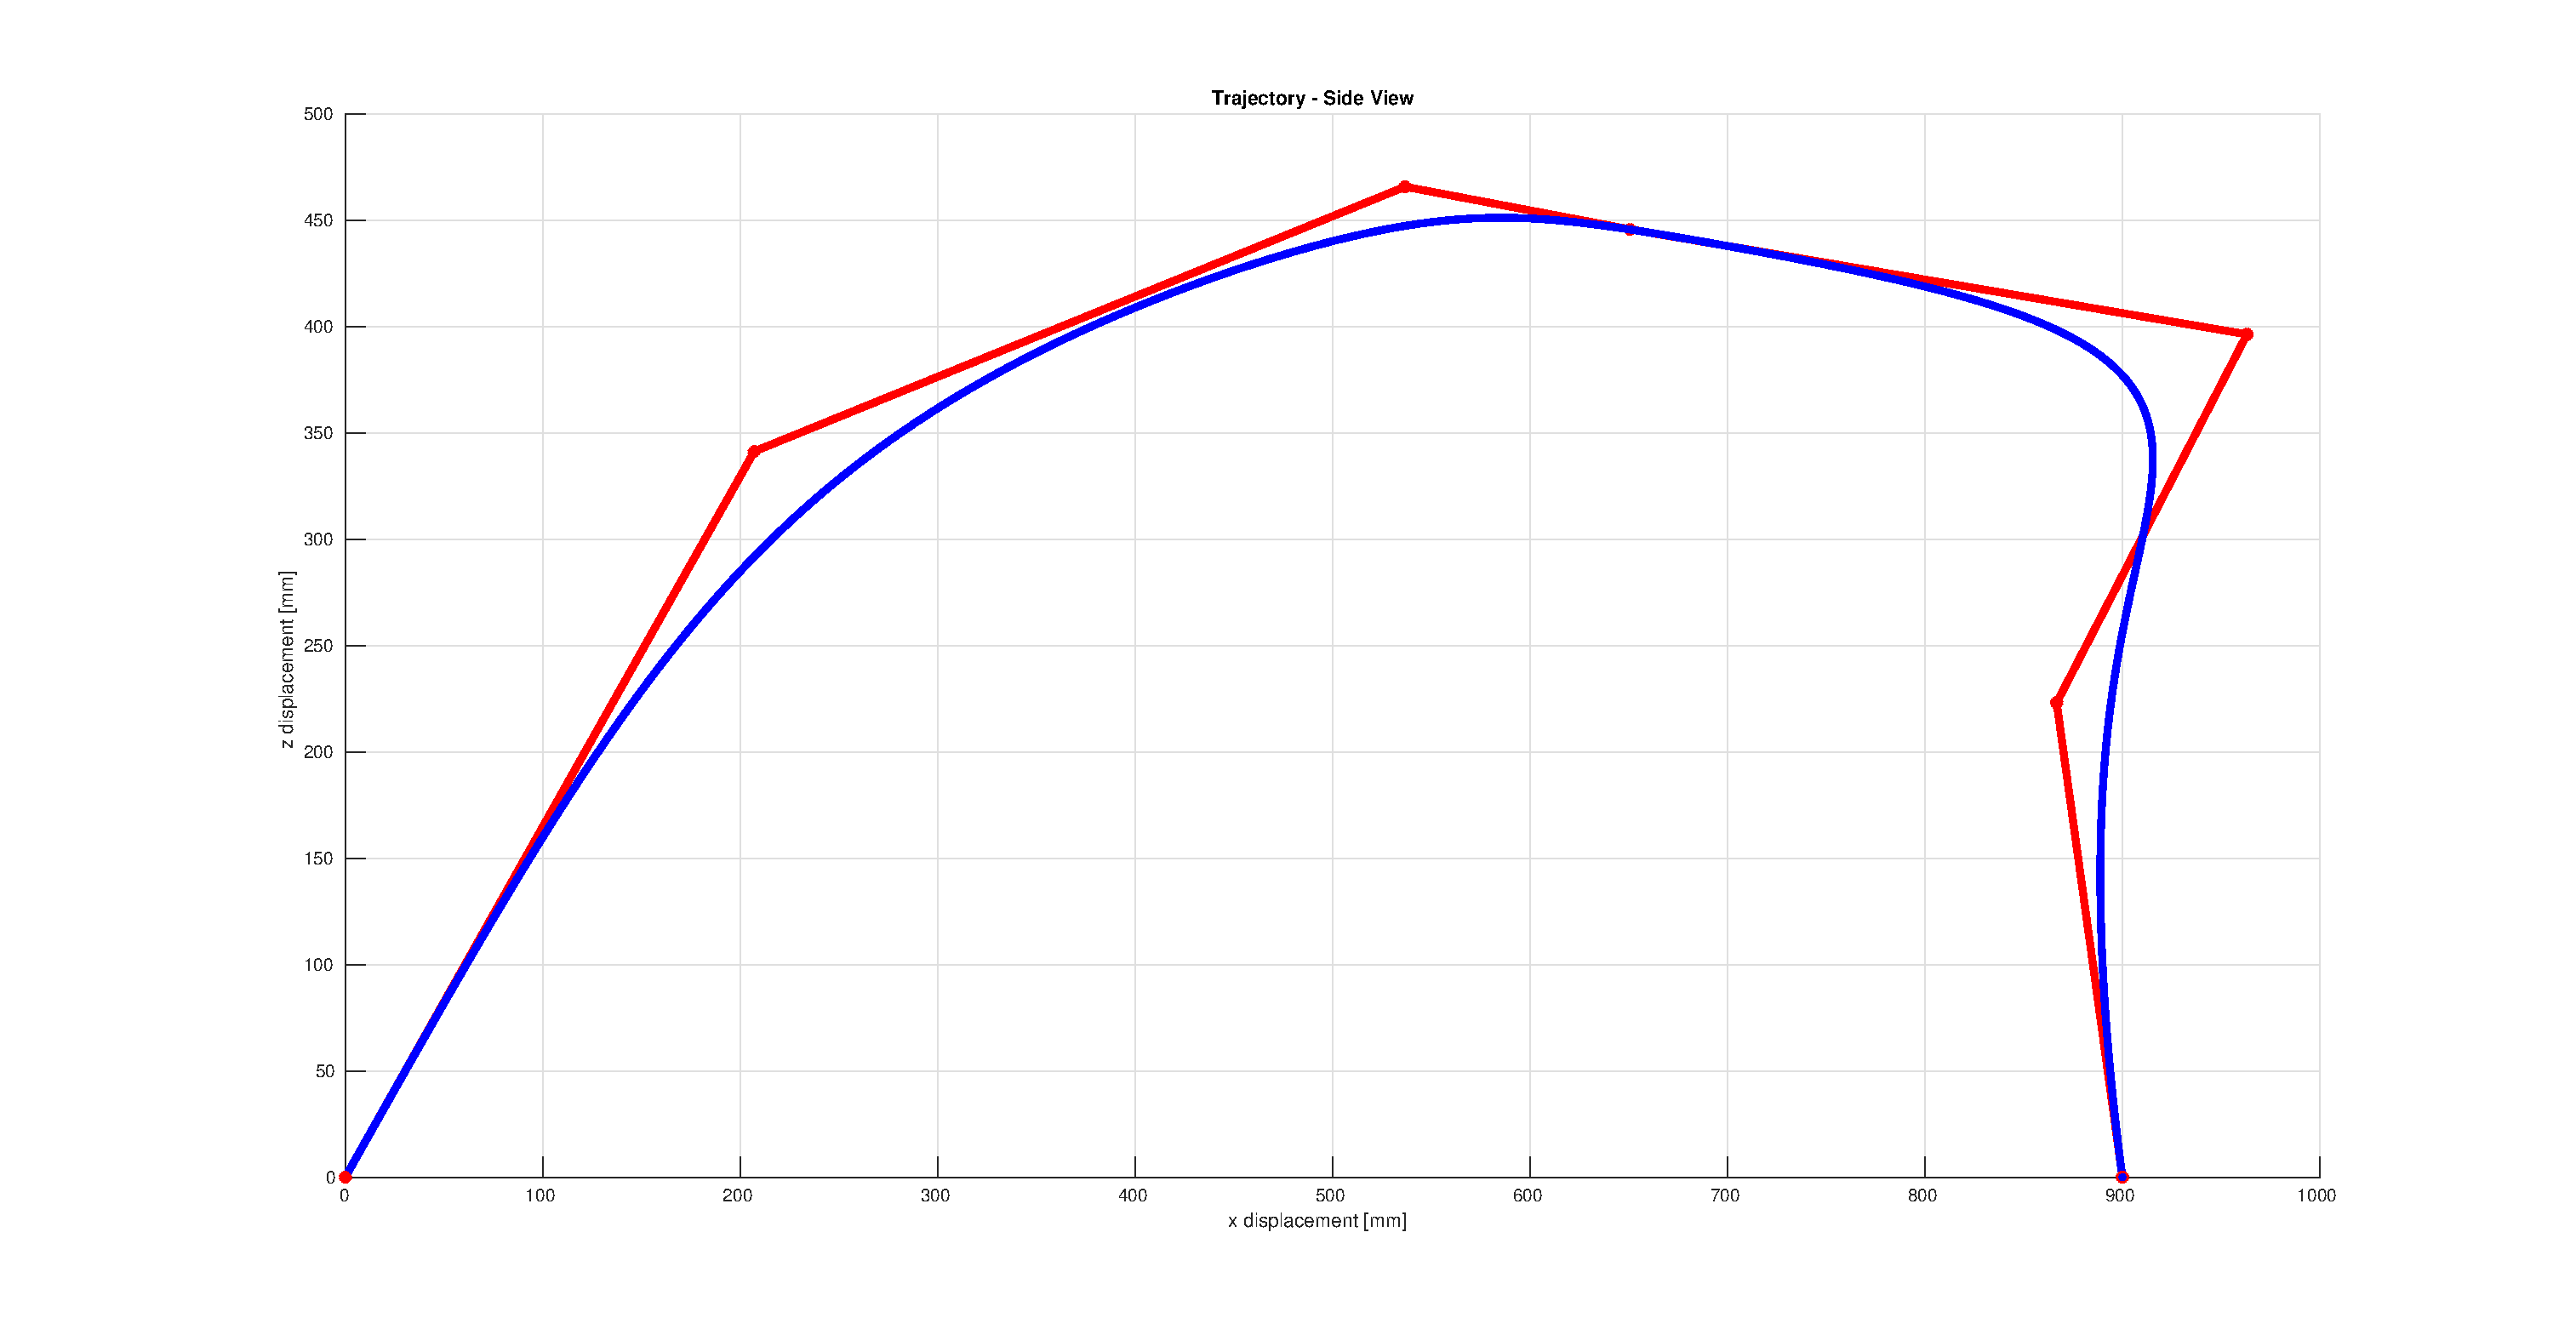
\includegraphics[height=0.45\linewidth, width=0.45\linewidth]{trajectory_simplify_subdivide_side.eps}
					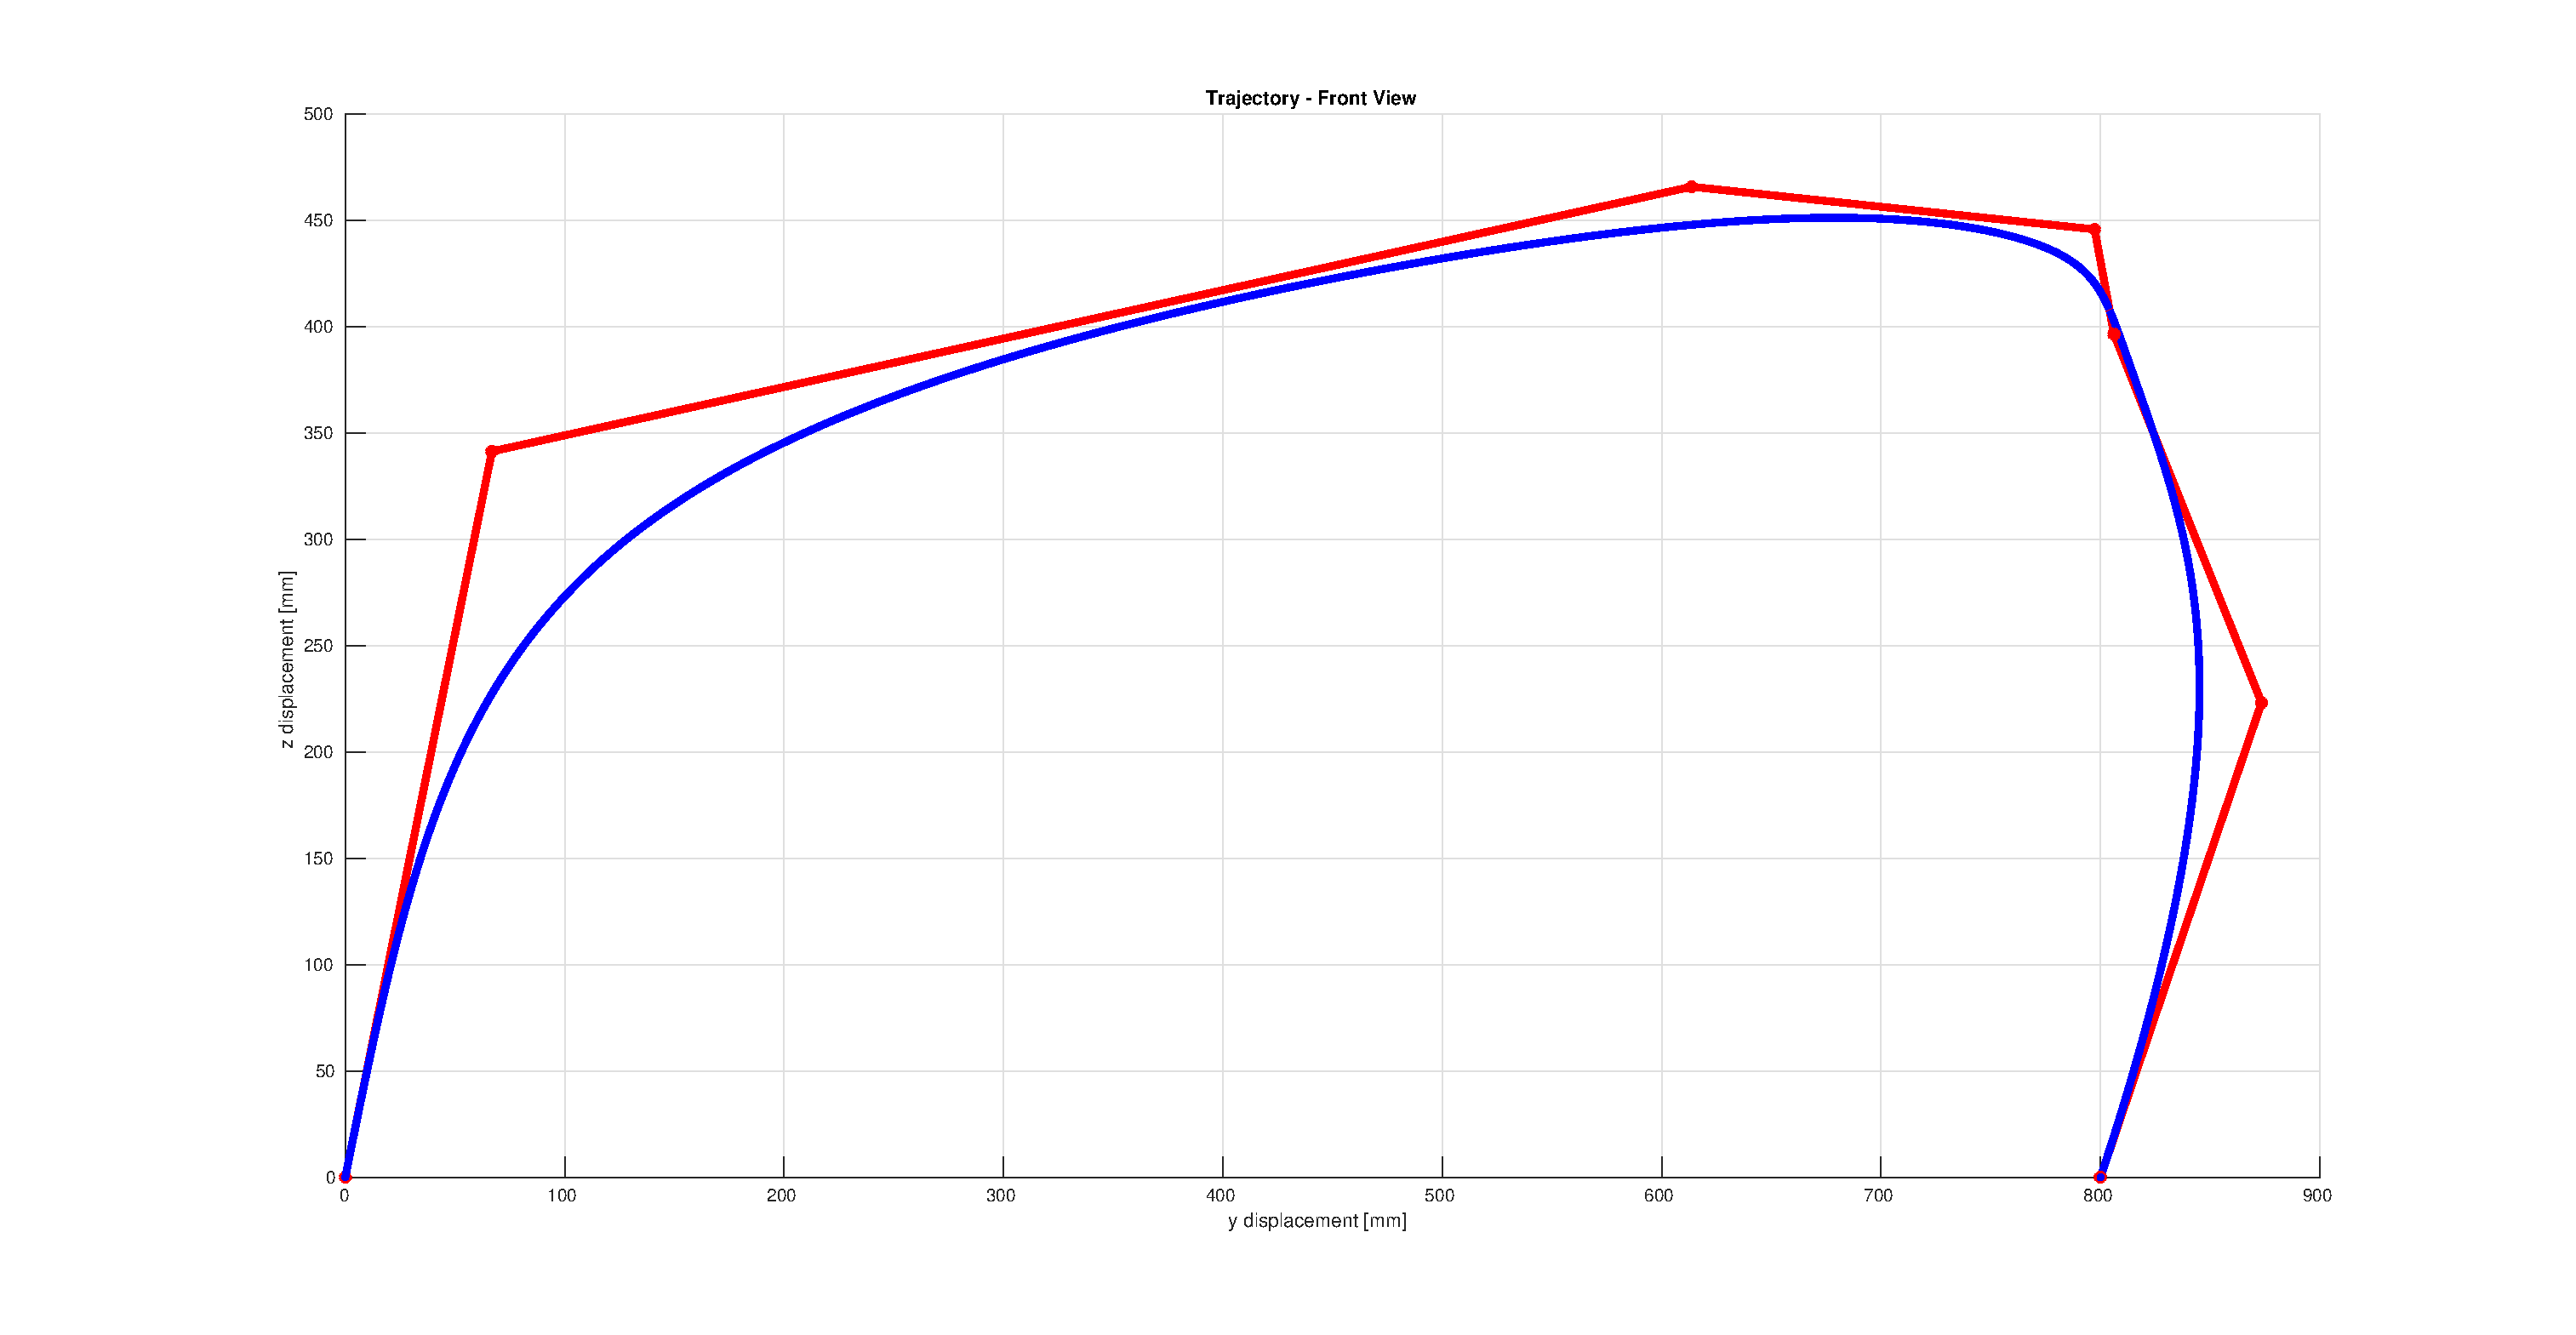
\includegraphics[height=0.45\linewidth, width=0.45\linewidth]{trajectory_simplify_subdivide_front.eps}
					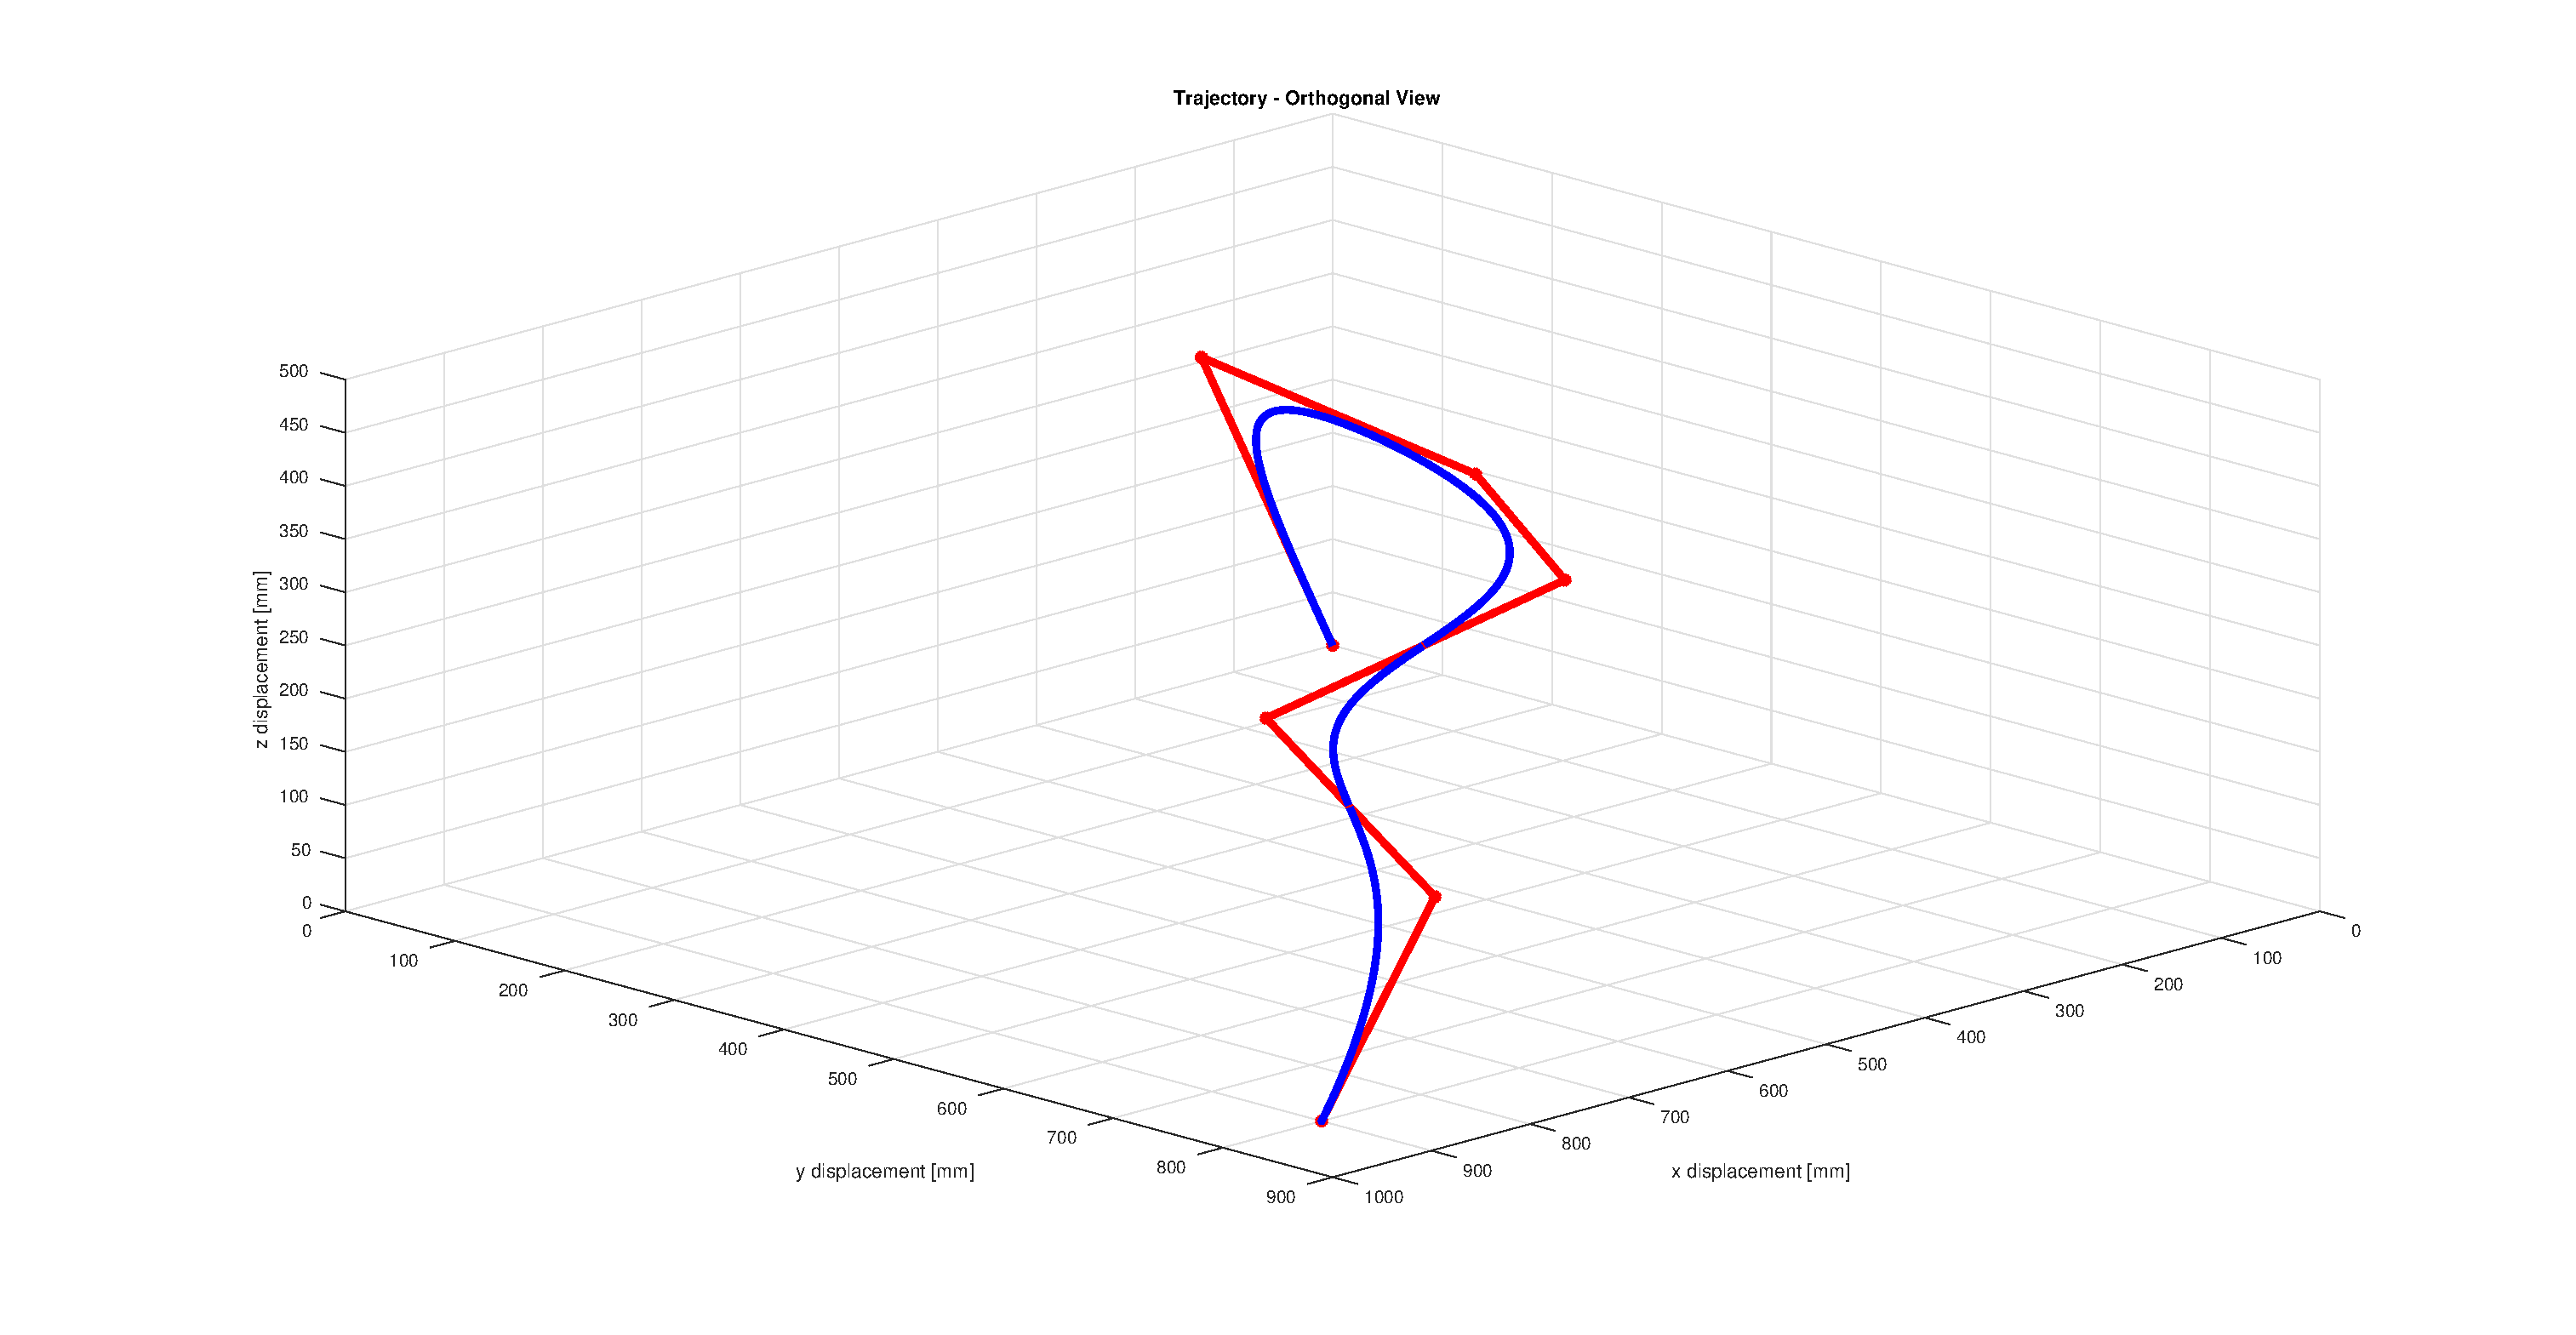
\includegraphics[height=0.45\linewidth, width=0.45\linewidth]{trajectory_simplify_subdivide_orthogonal.eps}
					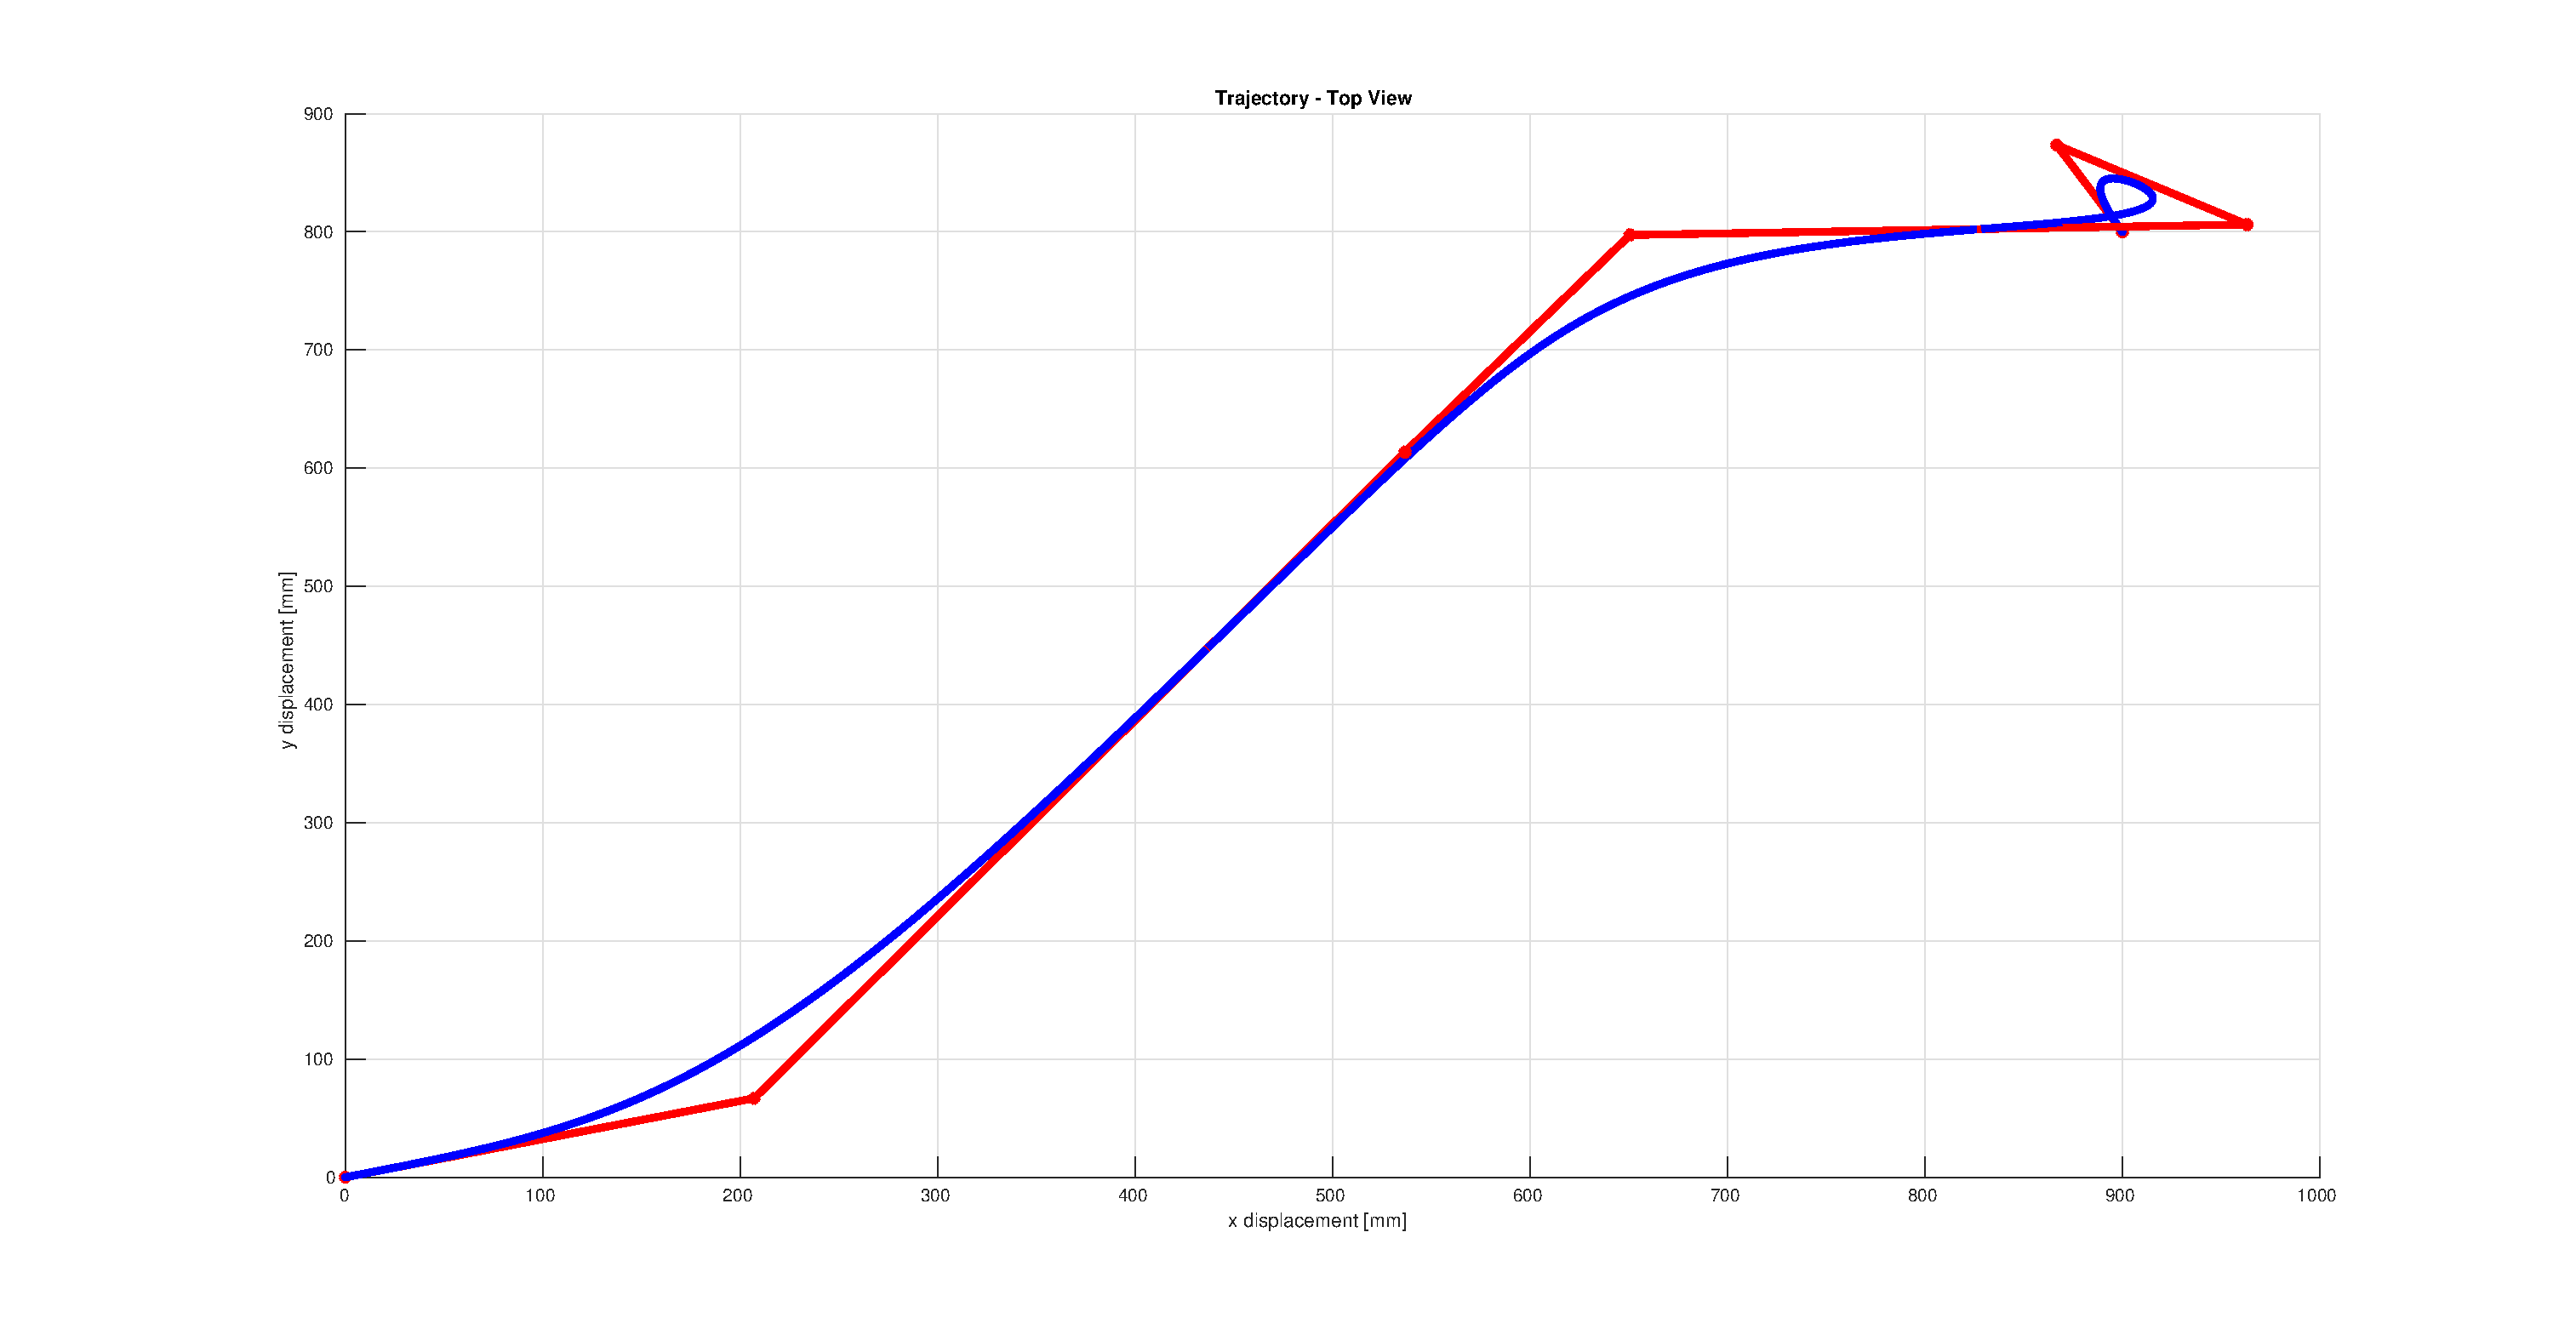
\includegraphics[height=0.45\linewidth, width=0.45\linewidth]{trajectory_simplify_subdivide_top.eps}
				\end{minipage}
				\caption{Sample Trajectory with Augmented $\setofposes$}
				\label{fig:sample_trajectory_with_augmented_set_of_poses}
			\end{figure}
	\end{columns}
\end{frame}

\begin{frame}
	\frametitle{Path-Planning Demo}

	\movie[
		height = 5cm,
		width = 5cm,
		externalviewer,
		showcontrols
	]
	{Demo}{./demos/demos/complex_rotation_avoid.mp4}
\end{frame}

\begin{frame}
	\frametitle{Motion Law}

	\begin{figure}[hb]
		\centering
		\def\svgwidth{0.5\textwidth}
		\import{res/img/}{motion_law_intuition.pdf_tex}
		\caption{Motion Law Construction}%
		\label{fig:motion_law_graphical_intuition}
	\end{figure}

\end{frame}

\begin{frame}
	\frametitle{Motion Law Sample Problem}
	\begin{figure}
		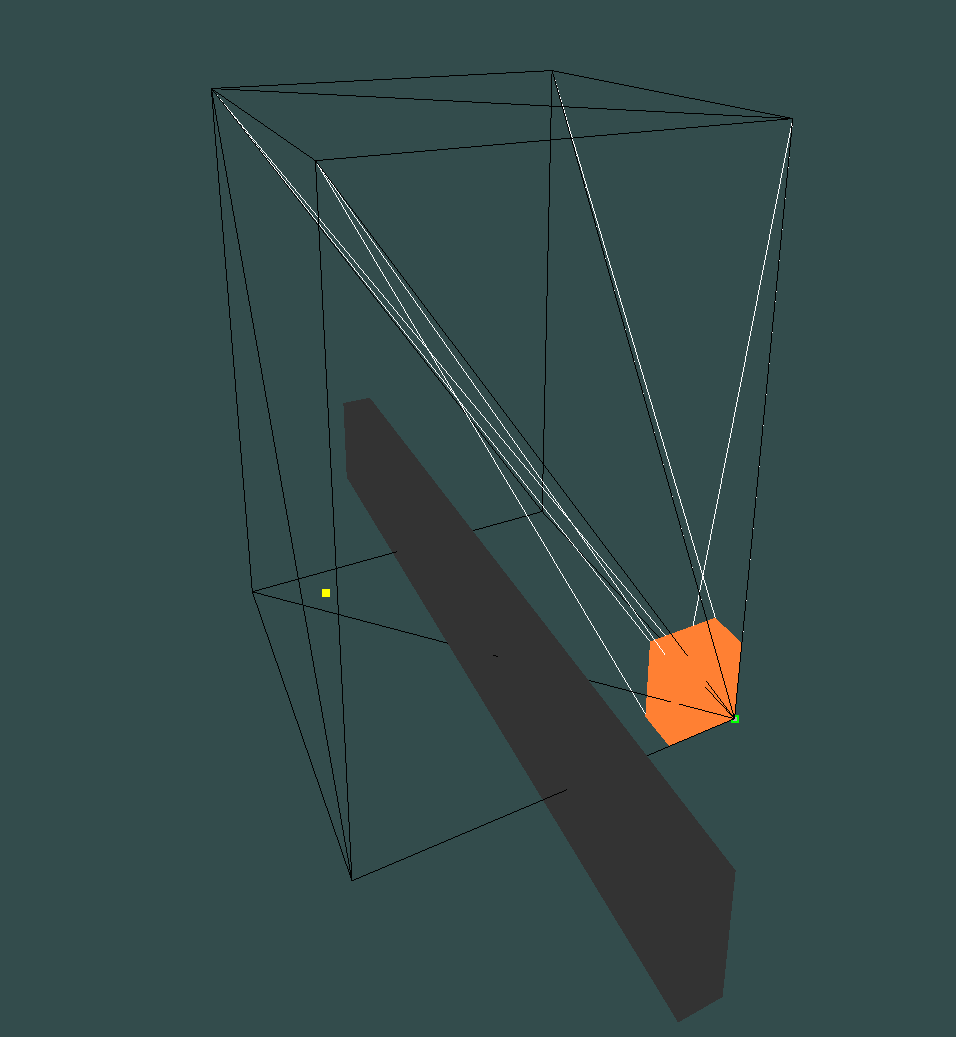
\includegraphics[height=0.75\textheight]{kinematic_scaling_base_problem}
		\caption{Sample Problem}
	\end{figure}
\end{frame}

\begin{frame}
	\frametitle{Motion Law Output}
	\begin{figure}[hb]
		\centering
		\begin{minipage}{0.45\textwidth}
			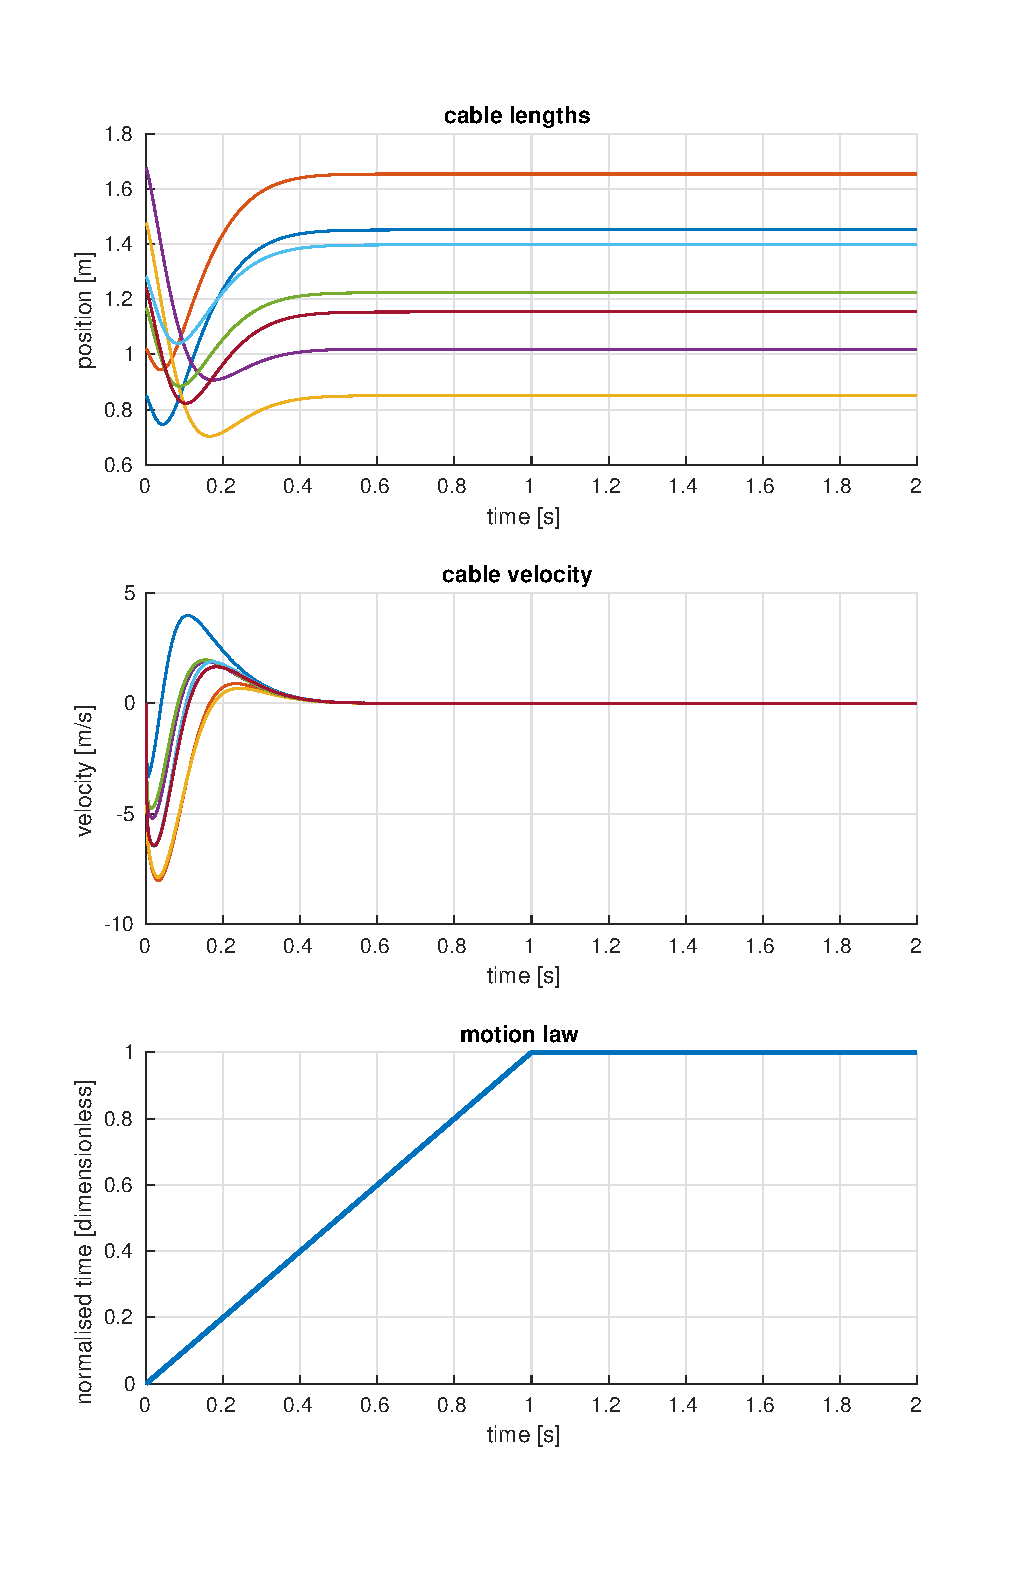
\includegraphics[width=\textwidth]{motion_law_linear}
		\end{minipage}%
		\begin{minipage}{0.45\textwidth}
			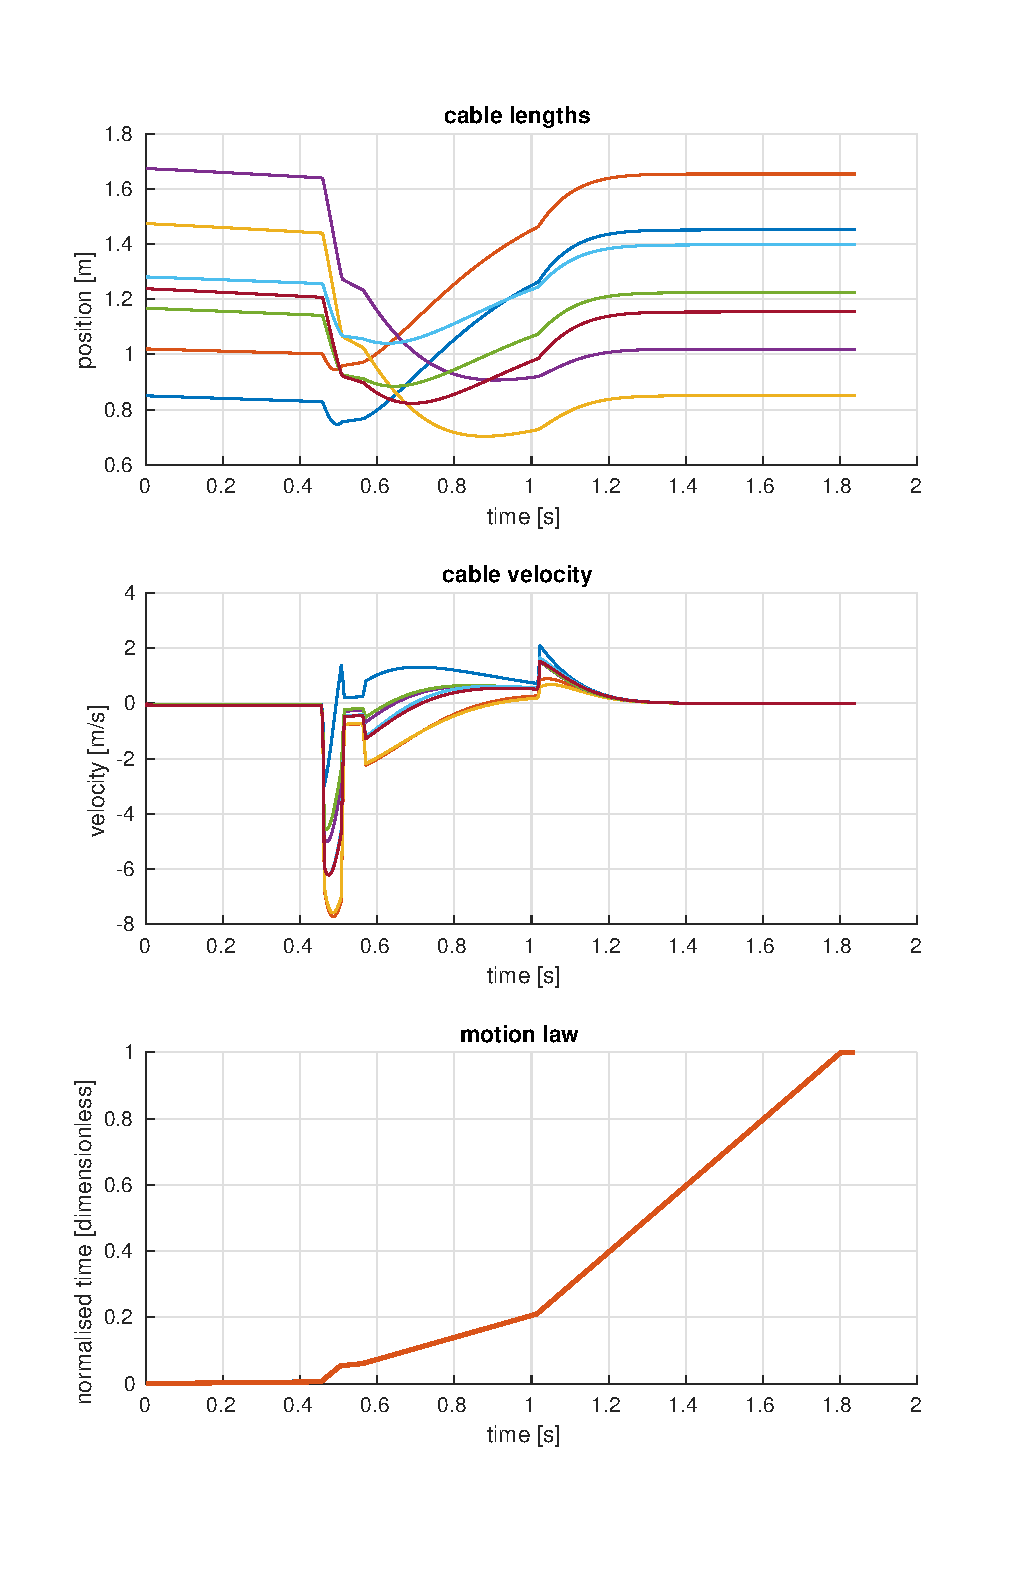
\includegraphics[width=\textwidth]{motion_law_deg_1}
		\end{minipage}
		\caption{No Motion Law (left) and Degree 1 (right) Motion Law}
		\label{fig:motion_law_lin_1}
	\end{figure}
\end{frame}
\begin{frame}
	\frametitle{Motion Law Output}

	\begin{figure}[hb]
		\centering
		\begin{minipage}{0.45\textwidth}
			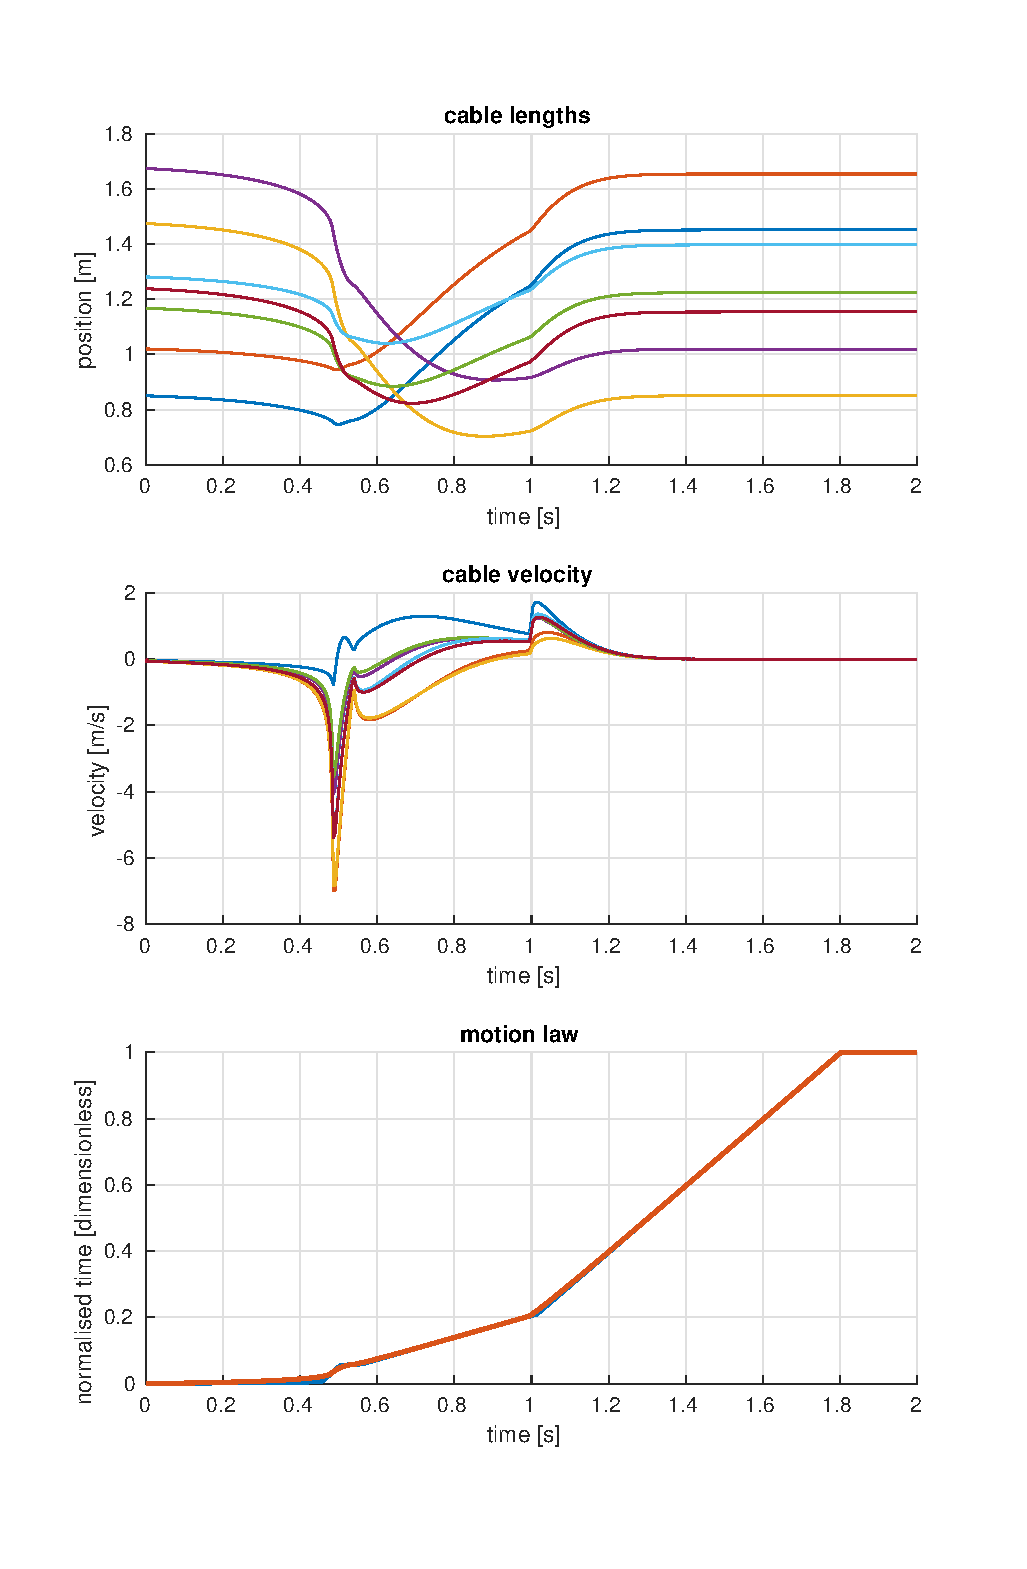
\includegraphics[width=\textwidth]{motion_law_deg_2}
		\end{minipage}%
		\begin{minipage}{0.45\textwidth}
			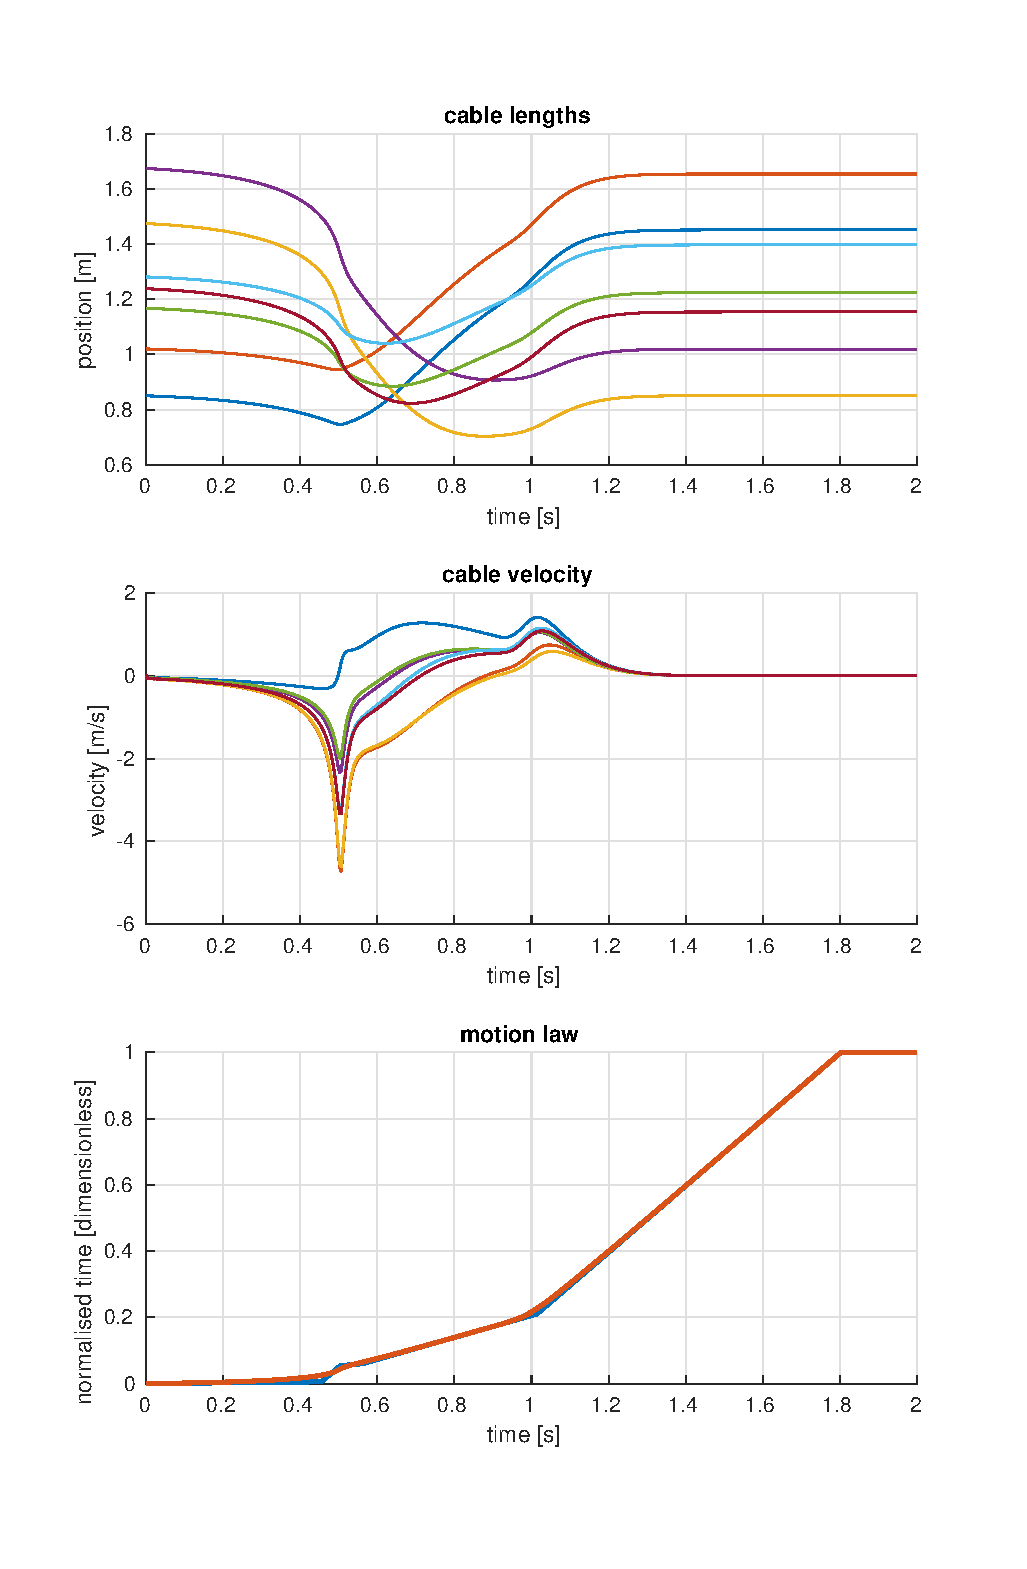
\includegraphics[width=\textwidth]{motion_law_deg_3}
		\end{minipage}%
		\caption{Degree 2 (left) and Degree 3 (right) Motion Law}
		\label{fig:motion_law_2_3}
	\end{figure}
\end{frame}

\begin{frame}
	\frametitle{Motion Law Output}

	\begin{figure}[hb]
		\centering
		\begin{minipage}{0.45\textwidth}
			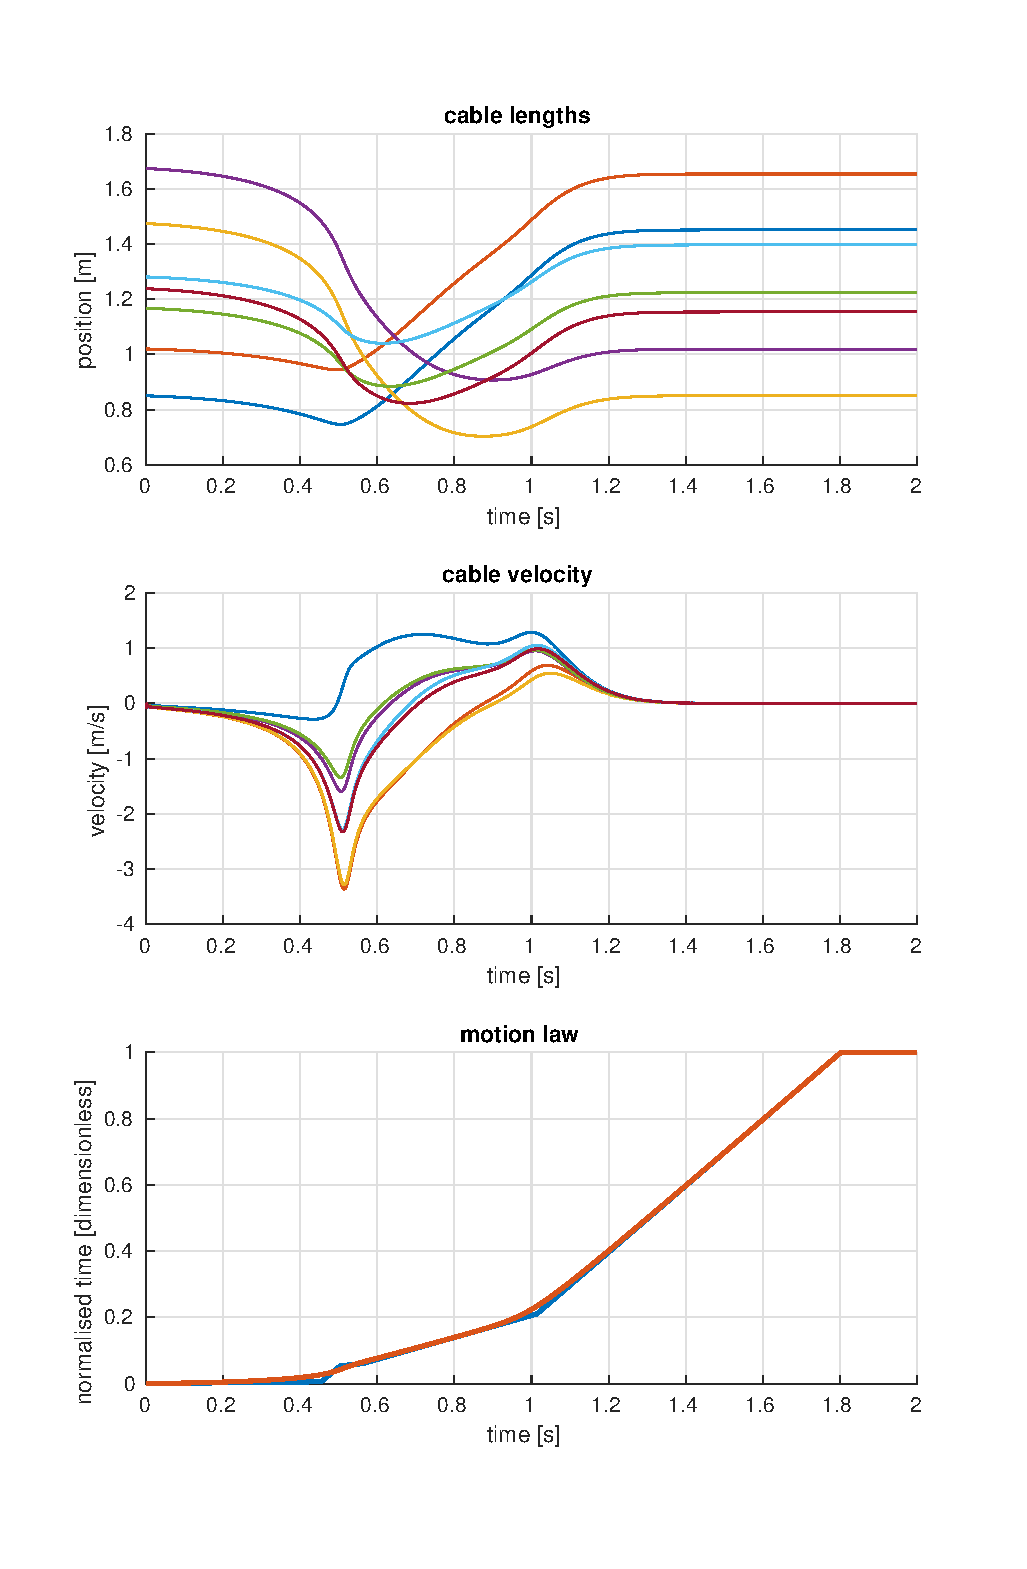
\includegraphics[width=\textwidth]{motion_law_deg_4}
		\end{minipage}%
		\begin{minipage}{0.45\textwidth}
			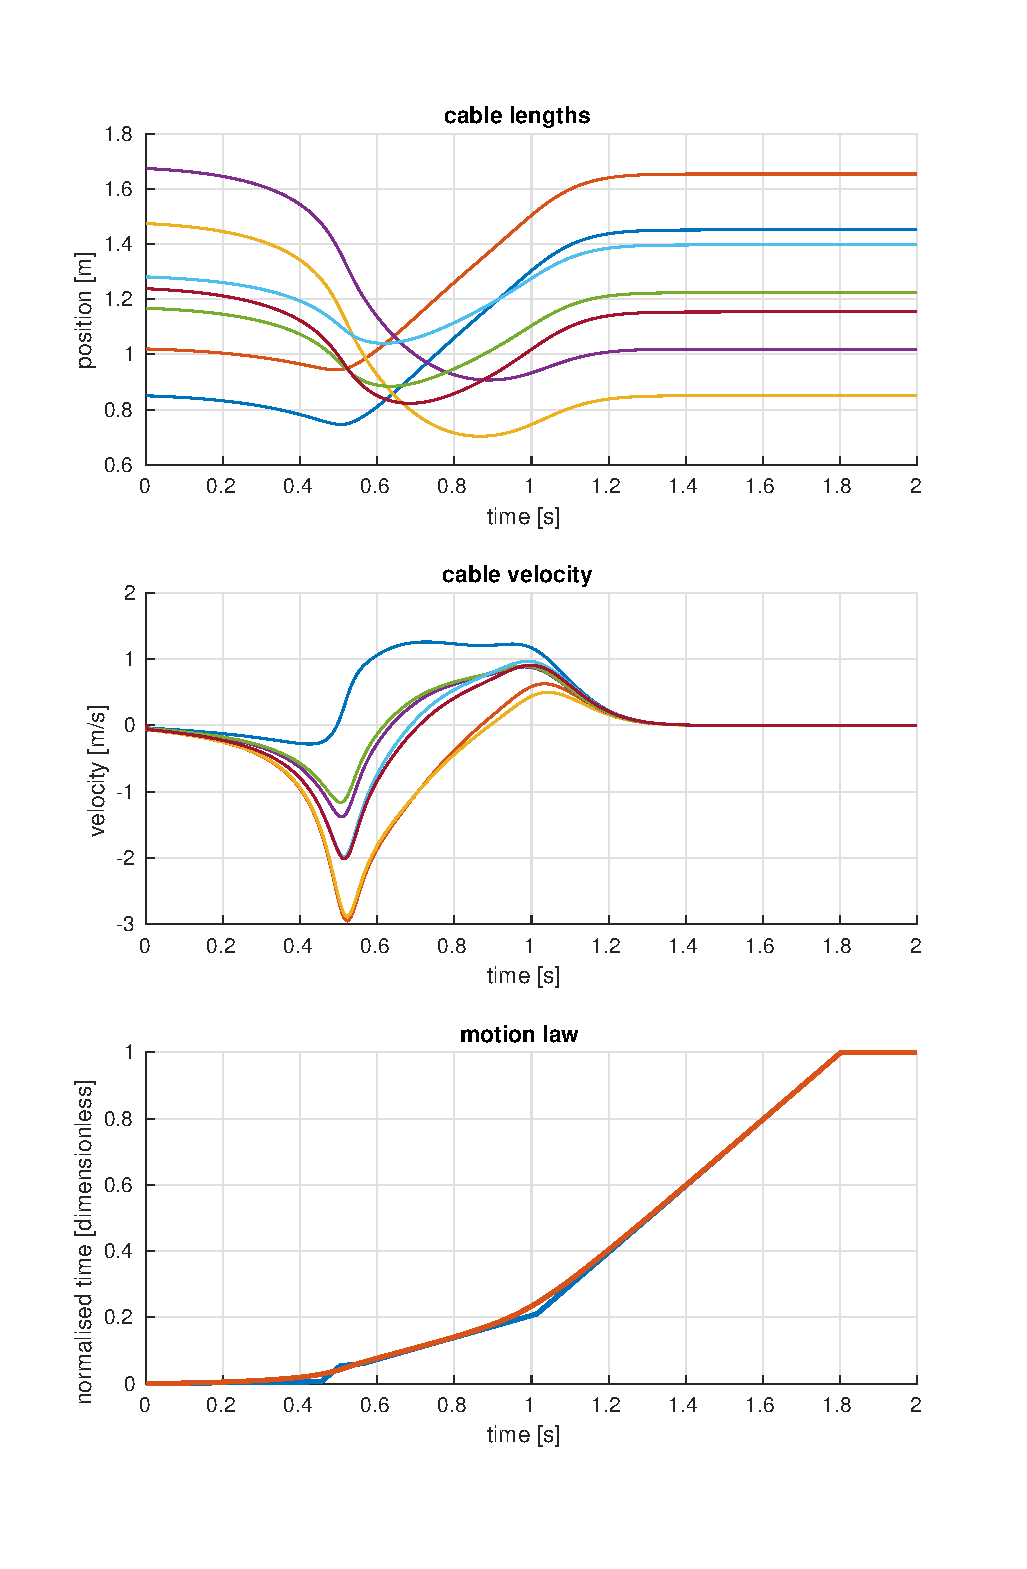
\includegraphics[width=\textwidth]{motion_law_deg_5}
		\end{minipage}%
		\caption{Degree 4 (left) and Degree 5 (right) Motion Law}
		\label{fig:motion_law_4_5}
	\end{figure}
\end{frame}

\begin{frame}
	\frametitle{Motion Law Output}

	\begin{figure}[hb]
		\centering
		\begin{minipage}{0.45\textwidth}
			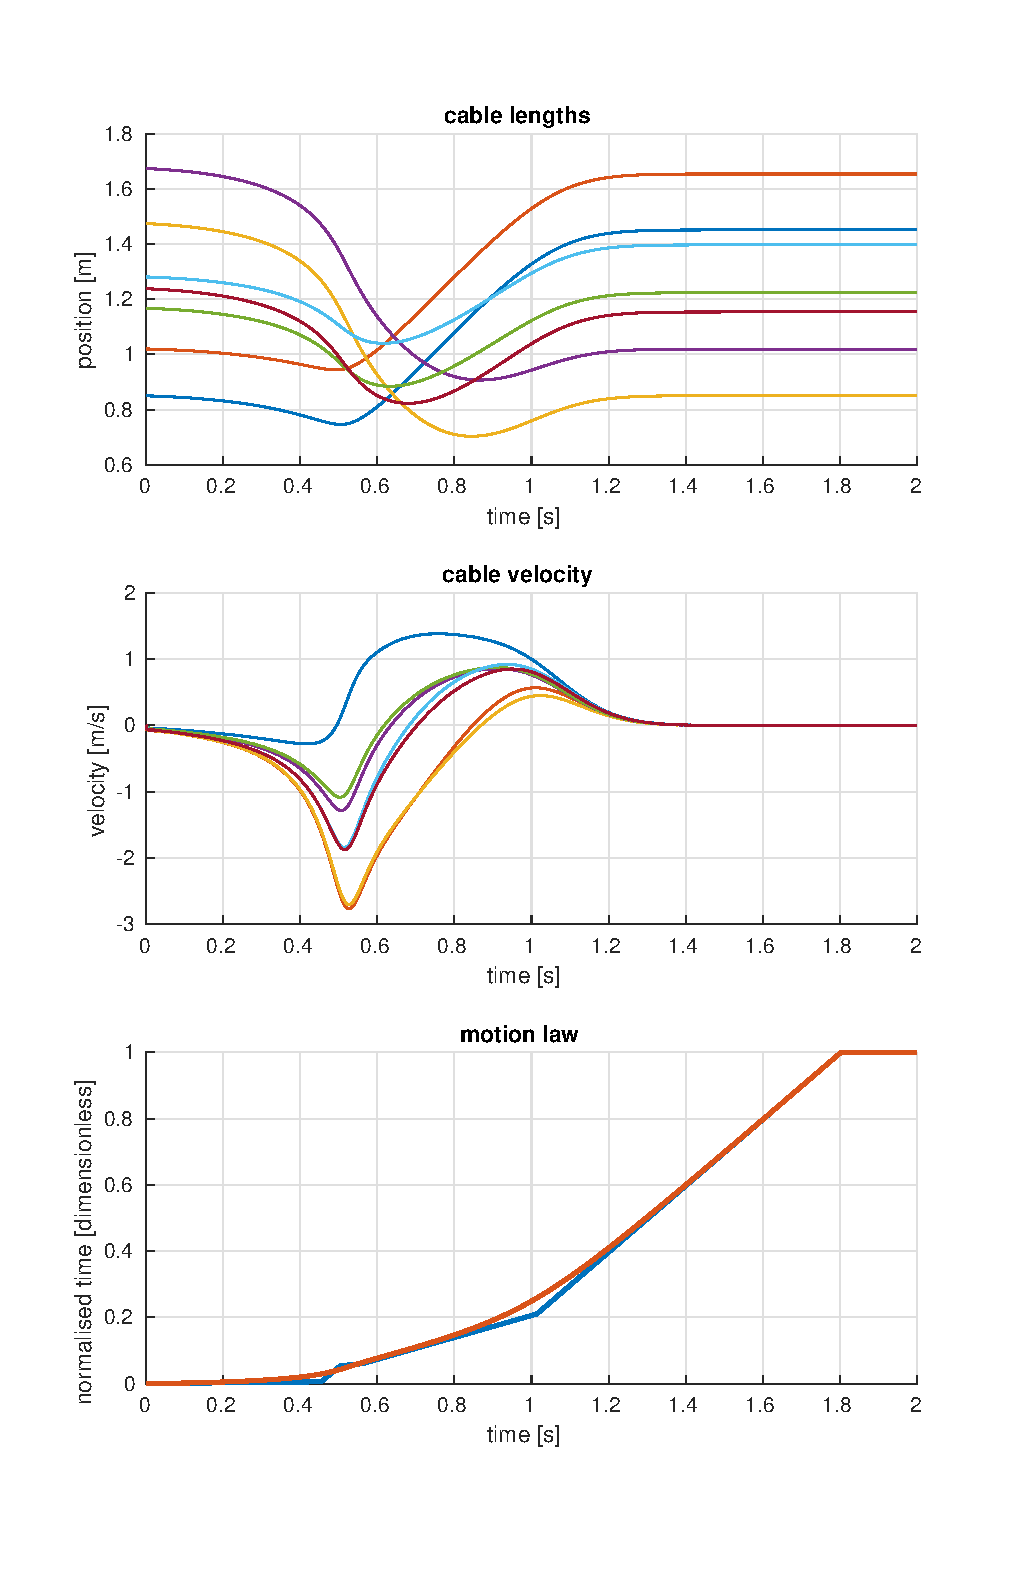
\includegraphics[width=\textwidth]{motion_law_deg_6}
		\end{minipage}%
		\begin{minipage}{0.45\textwidth}
			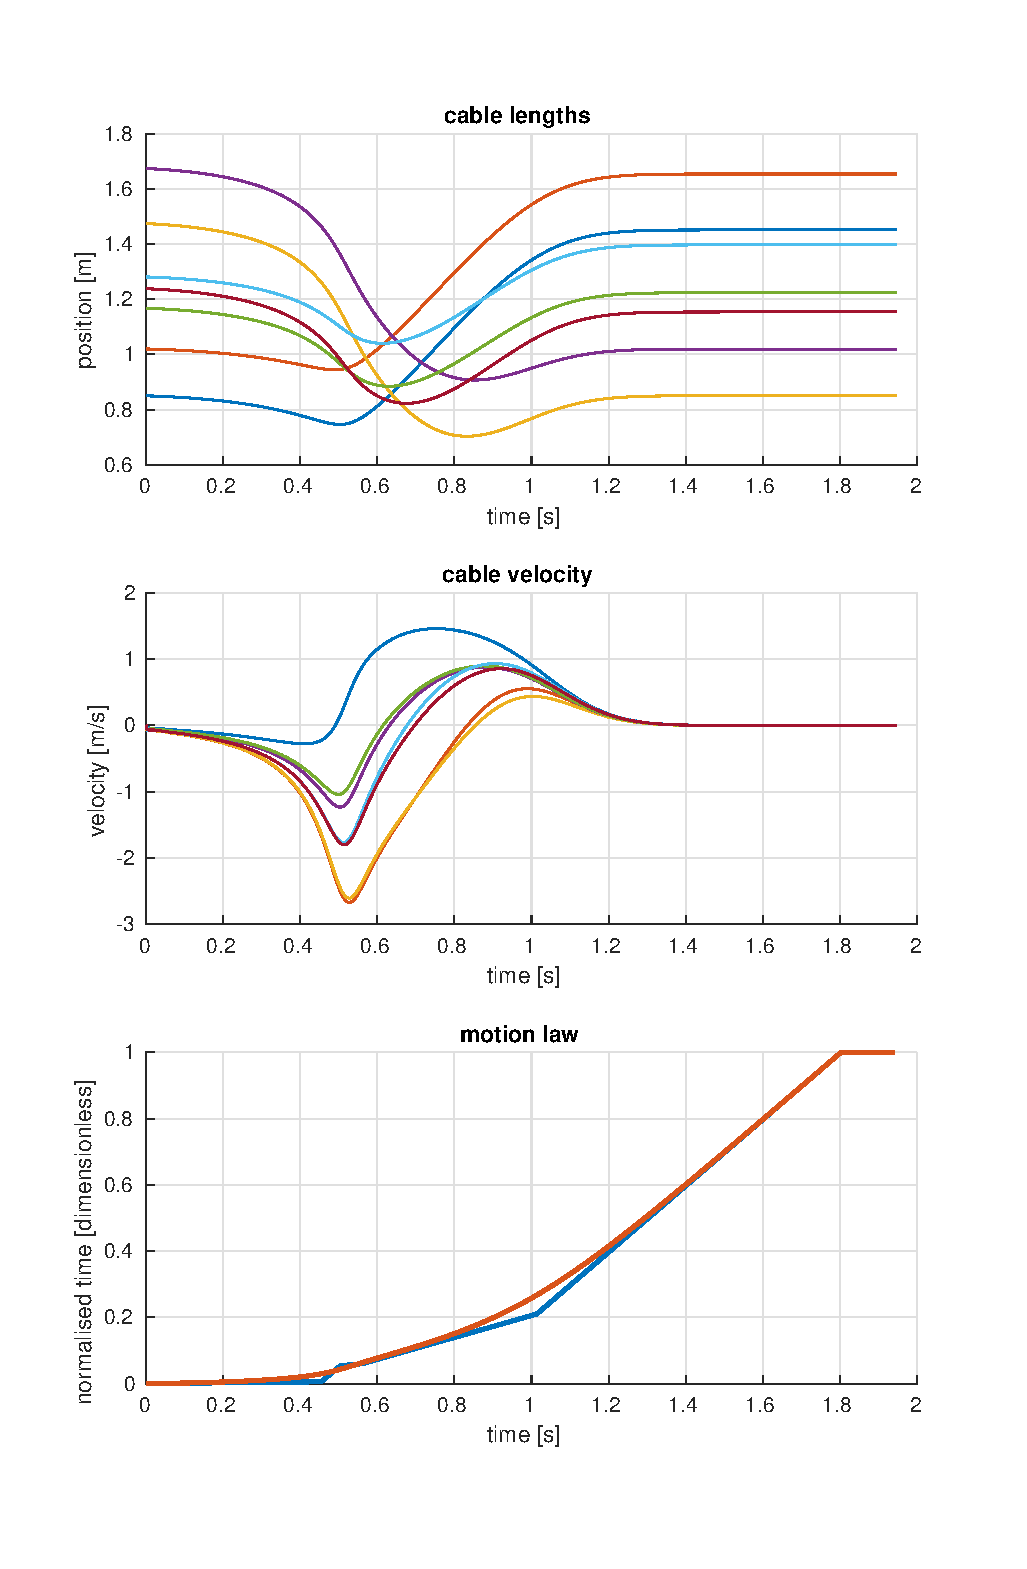
\includegraphics[width=\textwidth]{motion_law_deg_7}
		\end{minipage}%
		\caption{Degree 6 (left) and Degree 7 (right) Motion Law}
		\label{fig:motion_law_6_7}
	\end{figure}
\end{frame}
